% !TEX root = ../thesis-example.tex
%
\chapter[An investigation of Bayesian-$C_{\ell}$ Estimators applied to Galaxy Clustering]{An investigation of Bayesian Angular Power Spectra Estimators applied to Galaxy Clustering}\label{Chap:BPL}
%\chapter{}\label{sec:concepts}

\cleanchapterquote{It's f*cking science!\\
Just ask Albert Einstein, he invented space
}{Danny Sexbang}{(Dinosaur Laser Fight, Ninja Sex Party)}

\vspace*{\fill}

In this Chapter, I present an investigation for applications of a fully Bayesian methodology to generally estimate angular power spectra from data distributed on a sphere. It provides tools for optimal power spectrum estimation of to CMB temperature and CMB polarisation modes. Here, I try to extend it to galaxy clustering measurements with a final goal to extend it, in the future, to weak lensing convergence ($\kappa$), cosmic shear ($\gamma_1$ \& $\gamma_2$), and cross-correlations of all previous probes. In other words, the goal is to develop an that estimator works for any spin-0 fields, spin-2 fields, and cross-correlations. However, this method, presented in \cite{SreeThesis}, has not been tested in the context of galaxy surveys. The method makes use of a Guided Hamiltonian Sampling, a variant of the usual Hamiltonian Sampling, to sample from the spherical harmonics coefficients,$a_{lm}$, and the angular power spectra, $C_{\ell}$. The final marginalised $C_{\ell}$'s provides covariance matrices and uncertainties with no the need of simulated mocks due to the sampling nature of the problem. I applied this method to partial and full-sky simulations, including Euclid-like log-normal simulations and compared the results with a Pseudo Power Spectrum estimator.

\textit{The work presented in this Chapter is an extension of the work presented by \cite{SreeThesis}, investigating the many aspects of applying such method to galaxy surveys, instead of CMB measurements.}

\newpage

\section{Introduction}
With a plethora of new cosmological observations in the horizon, there is an increasing necessity in the field for the use of an unified framework to combine different probes. Surveys like DESI \citep{2016-DESI}, Euclid \citep{2011EuclidRedPaper}, COrE \citep{2011CoRE}, LSST \citep{LSST}, J-PAS \citep{JPAS} would directly benefit from combining Cosmic Microwave Background temperature \& polarisation with galaxy clustering and galaxy lensing observations. Recent studies have demonstrated the power of probing cosmological parameters using `3x2pt' statistics, using galaxy clustering, galaxy lensing and cross-correlations of both \citep{2017MNRAS.465.1454H, 2017arXiv170801530D}; or `5x2pt' statistics, CMB polarisation, galaxy clustering, galaxy lensing, and cross-correlations \citep{2016Nicola, 2017Nicola, Doux2017}. 

\qquad During the last decades in cosmology, an increasing adoption of Bayesian methods of analysis happened within the community.\footnote{See \cite{2017TrottaReview} for a review.} In this context, most of the estimators used to probe anisotropies in the Universe do not met the Bayesian criteria. Most of the 3x2pt and 5x2pt works cited in the last paragraph all take a frequentist approach, having each their different flaws and limitations. The approach presented in Chapter \ref{Chap:BOSS}, the Pseudo-$C_{\ell}$ estimator, has the advantage of being easy to implement as the effects of partial sky can be forward modelled into the theoretical framework  (see Section \ref{Sec:Theory}). However, such approach fails to meet the criteria for being an `optimal quadratic estimator'\footnote{Meaning that it is not a minimum-variance estimator, i. e. it does not saturate the Cram\'er-Rao lower bound \citep{MR0015748,cramer2016mathematical}.}; although, it is an unbiased estimator by construction (check Section \ref{Sec:Measurements} and \cite{Peebles1973}). Other estimators, like the Quadratic Maximum Likelihood (QML) estimator meet the criteria of being minimum variance and unbiased; however, it is not entirely Bayesian and does not include the use of priors. This also causes this method to be computationally expensive to implement at the same time that it assumes a Gaussian shape for the uncertainties, failing to correctly probe the skewed distribution around the low-$\ell$ modes.

\qquad The main interest in obtaining accurate and precise low-$\ell$ information from a Bayesian framework is motivated by probing primordial non-Gaussianities, via the $f_{nl}$ parameter, with galaxy surveys \citep{2004Bartolo-fnl, 2008Dalal-fnl,2011Hamaus-fnl,2014Boris-fnl}. Information about $f_{nl}$ is concentrated in the large scale modes of the power spectra of galaxies, the region usually dominated by cosmic variance -- an artefact of galaxy surveys being always limited by the number of modes that can be used to probe large scales. Properly probing the posterior distribution of the power spectrum of galaxies in large scales can be the missing key to go beyond the $\Lambda$CDM standard model of cosmology.

\qquad During a considerable amount of time in my PhD, I have worked in adapting a Bayesian-$C_{\ell}$ estimator to work with galaxy clustering -- as it was originally developed in \cite{SreeThesis} for power spectra estimation of CMB temperature and polarisation. The anisotropic nature of the Poissonian noise in galaxy clustering and the calculation of the Hessian as a part of a Guided Hamiltonian Monte-Carlo algorithm \citep{2013-GuidedHamiltonian} turned to be more complicated than it seemed. The goal in this project was to extend and test a general model for applying Bayesian methods to the problem of measuring power spectra from data distributed on a sphere. The methods developed can be applied to CMB temperature, CMB polarisation modes, galaxy clustering, weak lensing convergence ($\kappa$), cosmic shear ($\gamma_1$ \& $\gamma_2$), and cross-correlations of all previous probes. In other words, the estimator works for spin-0 fields, spin-2 fields, and cross-correlations of both. However, the method remains untested for weak lensing measurements. The results I present in this chapter are related only to measuring clustering $C_{\ell}$s and are focused mainly on the case for Euclid's future galaxy clustering catalogues.

\qquad This Bayesian approach is ideal to be applied in an experiment like Euclid. The Euclid Satellite will have outstanding photometric and spectroscopic redshift precision -- $\sigma^{\text{photo}}_z/(1+z) < 0.05$ and  $\sigma^{\text{spec}}_z/(1+z)< 0.001$, respectively. Euclid's experimental design was additionally construct to obtain extremely accurate shape measurements for cosmic shear. Developing a full Bayesian estimator for cross-correlations between spin-0 and spin-2 fields for Euclid would aid the collaboration towards achieving Euclid's science goals. This Chapter is a step towards this goal by studying how to apply this methodology to galaxy clustering measurements and to an Euclid-like simulation in an intermediate redshift range.

\qquad This Chapter is outlined as follows: Section \ref{Sec:BPL:Modeling} outlines the details for the Bayesian approach to obtain power spectra estimates for both spin-0 and spin-2 fields; Section \ref{Sec:BPL:Sampling} outlines the details on the sampling algorithm, the Guided Hamiltonian Sampler, GHS \citep{SreeThesis,2013-GuidedHamiltonian}; the following section, Section \ref{Sec:BPL:SimData}, gives details about the simulations used to test and validate this method with galaxy clustering; next, Section \ref{Sec:BPL:Investigations} performs several investigations related to the statistical nature of galaxy clustering and how to probe the angular power spectra of galaxies with a Bayesian-$C_{\ell}$ estimator, this is performed by analysing different simulations with different masks and signal-to-noise ratios, including Euclid-like cases; finally, the last section outlines future work and possibilities for extending this approach. 

% \begin{itemize}
% \item Talk more about DES
% \item Different estimators: MQL, PCL and their disadvantages
% \item Talk about the importance for small-$\ell$ -- $f_{nl}$
% \item No need for mocks
% \item Euclid case
% \end{itemize}

\section{Bayesian Approach to Measure the Angular Power Spectra}\label{Sec:BPL:Modeling}
In this section, I will establish the formalism towards expressing a generic Bayesian modelling for angular power spectra estimation for data distributed on a sphere. The formalism developed here can be applied to CMB temperature data ($T$), CMB polarisation data($\Theta_P$), galaxy clustering ($\delta_g$), and probes of weak gravitational lensing like cosmic shear ($\gamma$) and convergence ($\kappa$). As a natural extension of the generic method, this also applies to cross-correlations between all of the above observables. In other terms, this Bayesian method for $C_{\ell}$ estimation works for spin-0 and spin-2 fields, considering also cross-power spectra between these.

\qquad Section \ref{Sec:BPL:Spin-0_Form}, starts by developing a general formalism for spin-0 fields like galaxy overdensities, weak lensing convergence, and CMB temperature (based on a previous work by \cite{Taylor2008}). We then move to the Bayesian inference modelling of measuring angular power spectra for such fields. Next, on Section \ref{Sec:BPL:Spin-2_Form}, we extend this formalism for Spin-2 fields like CMB polarisation and weak lensing shear, finishing this Section with a formalism for the Bayesian inference of Spin-0 and Spin-2 angular power spectra estimation.


%--------------------------------------------------------------%
%                  SPIN-1 MODELLING
%--------------------------------------------------------------%
\subsection{Spin Zero Fields}\label{Sec:BPL:Spin-0_Form}
One may start the modelling by partitioning the sky into pixelised regions of equal area, $x_p$. For an underlying cosmological field, measurements can be described by a vector -- e.g. $T(x_p)$ for CMB temperature or $\delta_g (x_p)$ for galaxy overdensities. Let $\mathbf{\Theta} \equiv \Theta(\mathbf{x}_p)$ denote a general spin-0 data vector which can be represented in harmonic space in terms of the coefficients of a spherical harmonic expansion:

\begin{equation}
\Theta (\mathbf{x}_p) = \sum_{\ell=0}^{\ell_{max}}\sum_{m=-\ell}^{\ell}a_{\ell m}Y_{\ell m}(\mathbf{x}_p).
\label{Eq:Spin0Decomp}
\end{equation}
\noindent this basis, the measured signal in the sky can be decomposed in an underlying signal vector, $\mathbf{s}$, and a noise vector, $\mathbf{n}$; in a way that the data can now be written as $\mathbf{d=s+n}$. The measured signal and the underlying spin-0 field are related via a linear mapping that takes into account any observational effects like instrumental pointing, masking, and beam effects: $\mathbf{s = R\Theta}$. Following, the spherical harmonics formalism, the relation between signal and noise can be re-written with the use of Equation \eqref{Eq:Spin0Decomp} as
\begin{align}
\mathbf{d=RYa+n}\, ,
\label{Eq:DataDecomposed}
\end{align}
\noindent  where $\mathbf{Y} \equiv Y_{\ell m}(\textbf{x}_p)$ are the spherical harmonics eigen-functions of the Laplace-Beltrami operator \citep{2008DahlenSimons}, $\mathbf{a} \equiv a_{\ell m}$ are the spherical harmonics coefficients which obey the relation $a_{\ell m} = (-1)^{m}a^*_{\ell (-m)}$. Note that the noise is also represented in this basis as $\textbf{n} \equiv n_{\ell m}$. 

\qquad In this context, the spin-0 fields are assumed to be isotropic Gaussian random fields with zero mean, i.e, $\langle \textbf{a} \rangle = \langle \textbf{n} \rangle = 0$, and covariances can be defined as

\begin{align}
\label{Eq:DataCov} \mathbf{C} & \equiv \langle \textbf{a} \textbf{a}^T \rangle = C_{\ell}\delta_{\ell \ell'}\delta_{m m'}, \\ 
\label{Eq:NoiseCov} \mathbf{N} & \equiv \langle \textbf{n} \textbf{n}^T \rangle = N_{\ell}\delta_{\ell \ell'}\delta_{m m'} \, , 
\end{align}
\noindent for the signal and the noise respectively. In Equation \eqref{Eq:DataCov}, the set of coefficients $\{C_{\ell}\}$ define the angular power spectrum of spin-0 fields. More generally, let $C_{\ell}^{ij, pq}$ denote the cross-power spectrum where \textit{(i,j)} are redshift tomographic bins and \textit{(p,q)} are probes. \footnote{In what follows, however, I will suppress the notational dependence on \textit{i,\, j,\, p}, and \textit{q}.} Equally, $N_{\ell}$ in Equation \eqref{Eq:NoiseCov} is defined as the noise power spectrum. Finally, the data covariance can be expressed as a sum of the two above covariances

\begin{equation}
\textbf{D} = \textbf{C} + \textbf{N} \, .
\end{equation}

\subsubsection{Bayesian inference for spin-0 fields:}
\qquad Now, the formalism is sufficient so one can take a Bayesian approach to infer the angular power spectra of spin-0 fields using sampling techniques. This approach can be formulated as the posterior probability of obtaining the $\{C_{\ell}\}$ given the data vector, $\mathbf{d}$:

\begin{align}
\Pr (\{C_{\ell}\}|\mathbf{d}) \propto \mathcal{L} (\mathbf{d}|\{C_{\ell}\})\Pi(\{C_{\ell}\}).
\label{Eq:LikelFirstExpression}
\end{align}
\noindent where $\mathcal{L} (\mathbf{d}|\{C_{\ell}\})$ is the likelihood of the data given the true $\{C_{\ell}\}$ and $\Pi(\{C_{\ell}\})$ is a prior in the angular power spectra. In a first approach, the expression above becomes a Maximum Likelihood estimation \citep{1994Gorsky,1997Tegmark,Hobson2002,Efstat2004} if one sets the prior probability distribution function on the angular power spectrum to $\Pi(\{C_{\ell}\}) = 1$. 

\qquad Following \cite{Borrill1999,Hobson2002,Taylor2008}, as both signal and noise are assumed to have a Gaussian nature, one can write the likelihood of the data as
\begin{align}
\mathcal{L}(\mathbf{d}|\{C_{l}\}) = \frac{1}{(2\pi)^{N_d/2}|\mathbf{D}|^{1/2}}\exp \left(-\frac{1}{2}\mathbf{d}^T\mathbf{D}^{-1}\mathbf{d} \right)\, .
\label{Eq:LikelihoodSpin0}
\end{align}

\qquad The right hand side of Equation \eqref{Eq:LikelihoodSpin0} can be estimated in reasonable computational time for very low resolution data. As the data's resolution increases, the dimensionality of the data covariance matrix $\mathbf{D}$, and hence its storage and memory requirements, increase drastically. This method becomes extremely complicated to deal with due to expensive inversion of $\mathbf{D}^{-1}$ following by the calculation of its determinant. Therefore, for the resolutions I am aiming in this work, the likelihood estimation in equation \eqref{Eq:LikelihoodSpin0} becomes extremely expensive\footnote{It is possible to find methods that work around this matrix inversion problem, but the matrix size makes the linear algebra an extremely complicated task}. 

\qquad To overcome this issue, two possible roads can be taken regarding two different approaches. The first one is to approximate the likelihood, in some way, to avoid the one given by equation \eqref{Eq:LikelihoodSpin0}. These methods are far from being optimal and can bias the likelihood. A second approach would be to estimate the signal realisation full posterior distribution and the angular power spectrum using Monte Carlo techniques \citep{Taylor2008,AlmostBlackPearl2016}. The $\{ C_{\ell}\}$ coefficients can be estimated with a marginalisation over all signal realisations sampled in the posterior. 

\qquad The power spectra's posterior distribution can be simply obtained from sampling from the joint distribution of $\{C_{\ell}\}$ coefficients and the signal realisation, $\Pr(\{C_{\ell}\},\mathbf{a}|\mathbf{d})$, and marginalising over the spherical harmonic coefficients \citep{Eriksen2004,Wandelt2004,Taylor2008,AlmostBlackPearl2016}:
%\qquad Now, following the approach described by \cite{Eriksen2004}, \cite{Wandelt2004}, \cite{Taylor2008}, and \cite{AlmostBlackPearl2016}, the posterior distribution of the power spectrum, $\Pr (\{C_{\ell}\}|\mathbf{d})$, can be obtained by sampling from the joint distribution of power spectrum coefficients and signal realisation, $\Pr(\{C_{\ell}\},\mathbf{a}|\mathbf{d})$, and finally marginalising over the $\mathbf{a}$ coefficients:
%\RED{CHANGE THE ABOVE PARAGRAPH!!!}

\begin{align}
\Pr(\{C_{\ell}\}|\mathbf{d}) = \int\Pr(\{C_{\ell}\},\mathbf{a}|\mathbf{d})\text{d}\mathbf{a}.
\label{Eq:LikelihInt}
\end{align}
\noindent The integrand can be expanded using Bayes theorem,

\begin{align}
\Pr(\{C_{\ell}\},\mathbf{a}|\mathbf{d}) \propto \mathcal{L}(\mathbf{d}|\mathbf{a})\mathcal{L}(\mathbf{a}|\{C_{\ell}\})\Pi(\{C_{\ell}\}). 
\label{Eq:Posterior1}
\end{align}
\noindent Given the assumed Gaussian nature of the noise, one can express $\mathcal{L}(\mathbf{d}|\mathbf{a})$ with the aid of Equation \eqref{Eq:DataDecomposed}:
\begin{align}
\mathcal{L}(\mathbf{d}|\mathbf{a}) \propto \exp \left[ -\frac{1}{2} (\mathbf{d-RYa})^T \mathbf{N}^{-1}(\mathbf{d-RYa}) \right] .
\end{align}
\noindent Furthermore, since the signal is also Gaussian,

\begin{align}
\mathcal{L}(\mathbf{a}|\{C_{\ell}\}) \propto \frac{1}{\sqrt{|\mathbf{C}|}}\exp\left( -\frac{1}{2} \mathbf{a}^T\mathbf{C}^{-1}\mathbf{a}\right).
\end{align}
\noindent With use of Equation \eqref{Eq:DataCov} the expression above can the re-written as:

\begin{align}
\mathcal{L}(\mathbf{a}|\{C_{\ell}\}) \propto \prod_{{\ell}=2}^{{\ell}_{max}}\left(\frac{1}{C_{\ell}}\right)^{(2\ell+1)/2} \exp \left[ -\frac{(2\ell+1)}{2}\frac{\sigma_\ell}{C_{\ell}}\right]\, ,
\end{align}
\noindent with 
\begin{align}
\sigma_{\ell} = \frac{1}{2\ell+1}\sum_m|a_{\ell m}|^2 \, ,
\end{align}
\noindent being the power spectrum of the signal realisation.

\qquad Finally, two components now express the posterior distribution: an Inverse-Gamma signal likelihood, and a Gaussian noise likelihood. Assuming that the noise in pixel space is uncorrelated, the noise covariance matrix, $\mathbf{N}$, will be diagonal. Furthermore, the signal's covariance matrix, $\mathbf{C}$, given by Equation \eqref{Eq:DataCov} is now diagonal in harmonic space. In this space, the likelihood $ \mathcal{L}(\mathbf{d}|\mathbf{a} )$ can be computed in an easier way. In other words, estimating the full posterior in the integrand of Equation \eqref{Eq:LikelihInt} becomes a much simpler task than calculating the full posterior in the left hand side of Equations \eqref{Eq:LikelFirstExpression} and \eqref{Eq:LikelihoodSpin0}. This is the usual approach taken by most works in the literature about Bayesian $C_{\ell}$ estimators.


%--------------------------------------------------------------%
%                  SPIN-2 MODELLING
%--------------------------------------------------------------%
\subsection{Spin Two Fields}\label{Sec:BPL:Spin-2_Form}
This section extends the formalism developed in the previous section to spin-2 fields like CMB polarisation and cosmic shear. Spin-2 fields can be separated into two independent modes related to the Stokes parameters. The first one is a curl-free mode, related to even-parity solutions, known as the E-mode; the second mode, related to odd-parity solutions, is the B-mode. In the formalism discussed in this Chapter, it is fundamental to note that incomplete sky coverage introduces mixing of these E- and B-modes, requiring the estimator to optimally deal with such systematic effects. In this section, I will adopt the same formalism and notation as in many seminal papers in the literature, as in \cite{Seljak1997}, \cite{Taylor2008} and \cite{Hikage2011}.

\qquad Starting with the argument that spin-2 fields are linear, they can fully be described by a traceless $2 \times 2$ tensor using only two of the Stokes parameters, $Q$ and $U$. The third Stokes parameter is related to the spin-0 field from Equation \eqref{Eq:Spin0Decomp}; while the fourth and final parameter is assumed to be zero since there's no circular polarisation generated by Thompson scattering (in the CMB context) and it is well known that there's no circular polarisation arising from the lensing potential in the weak lensing context, \citep{2005astro.ph..9252S,2017SchpJ..1232440B}. In the case for CMB polarisation, the two Stokes parameters, $U$ and $Q$, are related to the $2\times 2$ intensity tensor, $I_{ij}$, as $Q=(I_{11}-I_{22})/4$ and $U=I_{12}/2$; while in the context of weak lensing shear, this relation simply translates into the two shear components, $Q=\gamma_1$ and $U=\gamma_2$.

\qquad The three non-vanishing Stokes parameters can now be defined by an orthonormal directional vector, $\hat{\mathbf{n}}$, with respect to spherical coordinates. These can be expanded using a spin-2 spherical harmonic basis, $_{\pm 2}Y_{\ell m}(\hat{\mathbf{n}})$, as 
\begin{align}
\label{eqn::chCmbPol_stokes_paras}
\Theta(\hat{\mathbf{n}}) &= \sum_{\ell m}a_{\ell m}\,Y_{\ell m}(\hat{\mathbf{n}}) \\
\left[ Q(\hat{\mathbf{n}})\pm iU(\hat{\mathbf{n}}) \right] &= \sum_{\ell m}\left(E_{\ell m}\pm iB_{\ell m} \right)\,_{\pm 2}Y_{\ell m}(\hat{\mathbf{n}})\, ,
\end{align}
%\left[ Q(\hat{\mathbf{n}})\pm iU(\hat{\mathbf{n}}) \right] &= \sum_{\ell m}a_{\pm 2,\ell m}\,_{\pm 2}Y_{\ell m}(\hat{\mathbf{n}})\, ,
%\noindent where the coefficients $a_{\pm 2,\ell m}$ can be related to the E- and B-modes coefficients $a_{\ell m}^E$ and $a_{\ell m}^B$ through
\noindent where the harmonic coefficients of the E- and B-modes can be estimated directly from the shear/polarisation fields via the $Q$ and $U$ Stokes parameters \citep{PolSpice2005,Hikage2011},
\begin{align}
E_{\ell m} & = \frac{1}{2}\oint d\Omega_{\hat{\mathbf{n}}} \left[ Q(\hat{\mathbf{n}}) + iU(\hat{\mathbf{n}}) \right]\,_2Y^*_{\ell m} + \left[ Q(\hat{\mathbf{n}}) - iU(\hat{\mathbf{n}}) \right]\,_{-2}Y^*_{\ell m} \, ,\\
B_{\ell m} & = -\frac{i}{2}\oint d\Omega_{\hat{\mathbf{n}}} \left[ Q(\hat{\mathbf{n}}) + iU(\hat{\mathbf{n}}) \right]\,_2Y^*_{\ell m} - \left[ Q(\hat{\mathbf{n}}) - iU(\hat{\mathbf{n}}) \right]\,_{-2}Y^*_{\ell m}\, .
\end{align}

\qquad The covariances between the spherical harmonics coefficients, also referred as the angular power spectra, are given by

\begin{align}
\label{eqn::chCmbPol_psTT}
\textbf{C}^{\Theta,\Theta}  \equiv & \langle a_{\ell m}^{*} a_{\ell'm'} \rangle  = C_{\ell}^{\Theta\Theta}\delta_{\ell\ell'}\delta_{mm'},\\
\label{eqn::chCmbPol_psEE}
\textbf{C}^{E,E} \equiv & \langle E_{\ell m}^{*} E_{\ell'm'} \rangle = C_{\ell}^{EE}\delta_{\ell\ell'}\delta_{mm'},\\
\label{eqn::chCmbPol_psBB}
\textbf{C}^{B,B} \equiv &\langle B_{lm}^{*} B_{l'm'} \rangle = C_{\ell}^{BB}\delta_{\ell\ell'}\delta_{mm'},\\
\label{eqn::chCmbPol_psTE}
\textbf{C}^{\Theta,E} \equiv & \langle a_{\ell m}^{*} E_{\ell'm'} \rangle = C_{\ell}^{\Theta E}\delta_{\ell\ell'}\delta_{mm'}, \\
\textbf{C}^{\Theta,B} \equiv &\langle a_{lm}^{*} B_{l'm'} \rangle = C_{\ell}^{\Theta B}\delta_{\ell\ell'}\delta_{mm'},\\
\textbf{C}^{E,B} \equiv &\langle E_{lm}^{*} B_{l'm'} \rangle = C_{\ell}^{EB}\delta_{\ell\ell'}\delta_{mm'}.
\end{align}

\qquad Note that the cross-power spectra $ C_{\ell}^{\Theta B}$ and $C_{\ell}^{EB}$ are expected to vanish since $B$ has the opposite parity to $\Theta$ and $E$, meaning that estimating these quantities are a good way of mitigating systematic contaminations. For generalisation purposes, each $\ell$-mode in the power spectra can be represented by a 3$\times$3 symmetric positive definite matrix given by a generic version of Equation \eqref{Eq:DataCov}:
\begin{equation}
\mathbf{C}_{\ell}=\left(
\begin{array}{ccc}
C_{\ell}^{\Theta\Theta} & C_{\ell}^{\Theta E} &  C_{\ell}^{\Theta B}\\
C_{\ell}^{\Theta E} & C_{\ell}^{EE} & C_{\ell}^{E B} \\
C_{\ell}^{\Theta B} & C_{\ell}^{E B} & C_{\ell}^{BB}
\end{array} \right)\, .
\label{Eq:Cl_blockDiag}
\end{equation}
\noindent If the spin-0 and spin-2 field's fluctuations are Gaussian, then the covariance matrix above is block-diagonal with each block being defined by $\mathbf{C}_{\ell}$. 

\subsubsection{Bayesian inference for spin-2 fields:}
I proceed now to outline the Bayesian modelling formalism for power spectra estimation of spin-2 fields. The following formalism is very similar to the probability modelling of spin-0 data in Section %\ref{Sec:Spin0-Inference}. 
\ref{Sec:BPL:Spin-0_Form}. Even so, for the sake of clarity, I will outline the modelling from the start once more. 

\qquad Consider the sky to be represented by observations of the Stokes parameters $\Theta,\, Q$ and $U$. The data vector $\mathbf{d}$ is the sum of a signal $\mathbf{s}$ and a noise $\mathbf{n}$ vectors; i. e. $\mathbf{d}=\mathbf{s}+\mathbf{n}$.  The signal can be related to the spherical harmonic coefficients, $\mathbf{a}$, through the spherical harmonic transforms presented. Hence, the data vector can be expressed as
\begin{equation}
\mathbf{d}=\mathbf{YBa}+\mathbf{n},
\end{equation}
\noindent where $\mathbf{B}$ represents the convolution of the window function, smoothing scale, pixel window function, or a beam -- any sort of systematic which introduces a characteristic scale in the analysis. To maintain generality, the signal covariance matrix $\mathbf{C}$ is a block diagonal matrix (Equation \ref{Eq:Cl_blockDiag}) meaning that there are no correlations between signal sphericial harmonic coefficients of different multi-poles. Thus, the $\bm{a}$ coefficients can be represented by
\begin{equation}
\mathbf{a} \equiv \mathbf{a}_{\ell m}=\left( a_{\ell m},E_{\ell m},B_{\ell m}\right),
\end{equation}

\qquad As in the previous section, sampling from the joint posterior distribution of the signal coefficients and the power spectra is much easier than from the distribution of the power spectra given the signal directly \citep{Wandelt2004,Larson2007,AlmostBlackPearl2016}. Using Bayes' theorem to re-write the posterior distribution in a similar way as in Equation \ref{Eq:Posterior1}, one has
\begin{equation}
\Pr(\mathbf{C}_{\ell},\mathbf{a}|\mathbf{d})=\mathcal{L}(\mathbf{d}|\mathbf{a})\mathcal{L}(\mathbf{a}|\mathbf{C}_{\ell})\Pi(\mathbf{C}_{\ell}).
\label{Eq:FullPost}
\end{equation}
The posterior distribution for the angular power spectra can be estimated by marginalising the joint probability distribution, $\Pr(\mathbf{C}_{\ell },\mathbf{a}|\mathbf{d})$, over the signal spherical harmonic coefficients $\mathbf{a}$. However, this argument only holds flat priors on the power spectra are assumed. Making this assumption, the marginalised posterior distribution can be represented by

\begin{equation}
\Pr(\mathbf{C}_{\ell}|\mathbf{d}) = \int \Pr(\mathbf{C}_{\ell},\mathbf{a}|\mathbf{d}) \text{d}\mathbf{a} .
\end{equation}


\qquad Once more, the noise is assumed to be a Gaussian realisation which makes the likelihood of data given the signal coefficients, $\mathcal{L}(\mathbf{d}|\mathbf{a})$, a Gaussian with a noise covariance matrix $\mathbf{N}=\langle\mathbf{nn}^{\mathrm{T}} \rangle$ (Equation \ref{Eq:NoiseCov}),
\begin{equation}
\label{eqn::chCmbPol_Prda}
\mathcal{L}(\mathbf{d}|\mathbf{a}) \propto \exp \left[-\frac{1}{2}(\mathbf{d}-\mathbf{YBa})^{\mathrm{T}}\mathbf{N}^{-1}(\mathbf{d}-\mathbf{YBa}) \right]\, ,
\end{equation}
which is very similar to the expression found in Section \ref{Sec:BPL:Spin-0_Form} for spin-0 zero fields. The same is true for the likelihood of the spherical harmonics given the $\mathbf{C}_{\ell}$s,
\begin{align}
\mathcal{L}(\mathbf{a}|\mathbf{C}) & = \prod_{\ell} \mathcal{L}(\mathbf{a} | \mathbf{C}_{\ell}) \\ 
& = \prod_{\ell}\frac{1}{\sqrt{|2\pi\mathbf{C}_{\ell}|}}\exp\left[-\frac{2\ell+1}{2}\mathrm{Tr}(\mathbf{C}_{\ell}^{-1}\boldsymbol{\sigma}_{\ell})\right],
\end{align}
\noindent which is an Inverse-Gamma distribution where $\boldsymbol{\sigma}_{\ell}$ is the ensemble of power spectra given by the $\mathbf{a}$ coefficients
\begin{equation}
\boldsymbol{\sigma}_{\ell} = \frac{1}{2\ell+1}\sum_m\,\mathbf{a}^{p}_{\ell m}\mathbf{a}_{\ell m}^{q}.
\end{equation}
\noindent Here \textit{p} and \textit{q} are indices which represent the fields: $\Theta$, $E$, and $B$. Note then that the $\boldsymbol{\sigma}_l$ is a $3\times 3$ matrix:

\begin{equation}
\label{eqn::chCmbPol_defSigma_l}
\boldsymbol{\sigma}_l=\left(
\begin{array}{ccc}
\sigma_{\ell}^{\Theta\Theta} & \sigma_{\ell}^{\Theta E} & \sigma_{\ell}^{\Theta B} \\
\sigma_{\ell}^{\Theta E} & \sigma_{\ell}^{EE} & \sigma_{\ell}^{EB} \\
\sigma_{\ell}^{\Theta B} & \sigma_{\ell}^{EB} & \sigma_{\ell}^{BB}
\end{array} \right).
\end{equation}

\qquad Naturally, this formalism, as well as the one in \ref{Sec:BPL:Spin-0_Form}, accounts for the case where one has several tomographic redshift bins with different galaxy tracers and observational probes. In order to simplify the notation, as mentioned in Sec. \ref{Sec:BPL:Spin-0_Form}, we decided to leave the index related to the tomographic bins and probes out of the formalism described above.

%--------------------------------------------------------------%
%                   SAMPLING DETAILS
%--------------------------------------------------------------%
\section{Sampling Details}\label{Sec:BPL:Sampling}
The objective in this section is to describe the necessary steps to efficiently sample from the signal and power spectra realisation's joint posterior for high resolution data. Here, I will review and present an extension of the previously mentioned Hamiltonian Sampling (see Section \ref{Sec:Sampling}). This extension, called Guided Hamiltonian Sampling (GHS), allows to effectively explore high dimensional posterior distributions \citep{SreeThesis,2013-GuidedHamiltonian}. Naturally, one can simply chose to use any other sample of their preference as long as it is capable to provide an accurate estimate of the power spectra coefficients. For example, a seminal paper by \cite{Wandelt2004} uses Gibbs sampling \citep{Geman1984,Casella1992} to exploit the generation of samples using the conditional distributions $\mathcal{L}(\mathbf{a}|\textbf{C}_{\ell},\mathbf{d})$ and $\mathcal{L}(\textbf{C}_{\ell}|\mathbf{a},\mathbf{d})$ in a much simpler fashion than if one tries to sample from the full posterior distribution $\Pr(\mathbf{a},\textbf{C}_{\ell}|\mathbf{d})$ -- like mentioned in the previous sections.

\qquad The conditional distribution $\mathcal{L}(\mathbf{a}|\textbf{C}_{\ell},\mathbf{d})$ is a multi-variate Gaussian and $\mathcal{L}(\textbf{C}_{\ell}|\mathbf{a},\mathbf{d})$ is an Inverse-Gamma distribution. This method, proposed by \cite{Wandelt2004}, alternately draws samples from these conditional distributions of $\mathbf{a}$ and $\textbf{C}_{\ell}$:

\begin{align}
\mathbf{a}^{i+1} &\longleftarrow\Pr(\mathbf{a}|\textbf{C}_{\ell}^i,\mathbf{d}), \nonumber \\
\textbf{C}_{\ell}^{i+1} & \longleftarrow\Pr(\textbf{C}_{\ell}|\mathbf{a}^{i+1},\mathbf{d}).\nonumber
\end{align}
Sampling from these distributions have a few advantages and complications. The Gaussian distribution is extremely simple to sample but computationally expensive, while the Inverse-Gamma distribution is not trivially sampled from but computationally simple. With increasing data resolution, like for surveys such as Euclid \citep{2011EuclidRedPaper}, sampling from a multivariate Gaussian becomes extremely time consuming due to the covariance matrix not necessarily being diagonal and having a high dimensionality. It is fundamental to bear in mind that the posterior distribution of the power spectrum estimations is typically uni-modal in a high-dimensional space ($\mathcal{O}(10^{4}-10^{7})$) \citep{Taylor2008,Wandelt2004}. This, naturally, requires the sampler not only to generate fast samples from this uni-modal probability distribution, but also to be efficiently scalable with a large dimensional space. 

\qquad From the uni-modality nature of the power spectra measurements, this probability distribution function can be approximated by a Gaussian. For the GHS, this Gaussian approximation can be defined by the Hessian of the posterior at the peak and will be used to `guide' the sampler -- which allows the sampler to draw samples from the relevant parts of the distribution. This `guiding' is fundamental to effectively sample from high dimension posteriors and it ensures that the sampler explores all of the posterior distribution, resulting in accurate statistical measurements once it's converged. After this Gaussian distribution approximation is achieved, one performs sampling in the principal coordinates in order to properly sample any correlation between the sampled parameters in the posterior distribution. 

\qquad Even for very high dimensional posteriors and non-Gaussian shaped posteriors, this algorithm efficiently generates samples as long as a peak is present. The next section will outline the HCM and how to extend it to become a GHS.

%---------------------------------------------------------------%
%                     GUIDED HAMILTONIAN SAMPLING 
%---------------------------------------------------------------%
\subsection{Guided Hamiltonian Sampling}\label{Sec:BPL:GHS}
Seminal works in the literature, like \cite{Hanson2001,Taylor2008}, used HMC to sample from high dimensional posteriors with around $10^6$ parameters. However, this method contain a complication related to searching for the perfect level of fine-tuning of free parameters in the sampler -- basically, one mass parameter for each dimension considered in the problem, according to the method implemented by \cite{Taylor2008}. Some subsequent work suggests pre-determining these free parameters for each specific problem. The objective here is to outline a robust sampling technique that can waive some of the fine-tuning facets of HMC sampler.

\qquad As mentioned in the previous section, GHS uses the Hessian at the peak of the posterior distribution to aid the sampler to probe effectively the multi-dimensional distribution. Using an eigen-decomposition of the Hessian at the peak, one can acquire information about the principal coordinates in which to sample from, achieving very high sampling efficiency.

\qquad Here, the starting point will be the formalism developed in \cite{Taylor2008,2013-GuidedHamiltonian} and summarised in Section \ref{Sec:Sampling} for the Hamiltonian Monte-Carlo sampler. To provide a complete discussion on the matter, I will briefly review a few important characteristics on HMC so the a comprehensive formalism on sampling from the principal coordinates can be outlined. The HMC method starts by considering the potential energy,$\psi$, of a posterior distribution, $\Pr(\bm{x})$, as
\begin{equation}
\label{eqn::ch1_log_post}
\psi(\mathbf{x})=-\log\Pr(\mathbf{x}).
\end{equation}
The Hamiltonian of the system can be expressed by
\EQ{}{
\mathcal{H} = \sum_i^N\frac{p_i^2}{2m_i} + \psi(\bm{x}) \, .}
where the extra parameters in the kinetic energy, $m_i$ and $p_i$, eventually can  be treated as nuisance parameters. Samples will be drawn from a distribution proportional to the posterior and a Gaussian distribution,
\begin{equation}
\label{EQ:BPL:HMC_ExpH}
\exp(-\mathcal{H})\propto \Pr(\bm{x})\prod_i^N\exp\left(-\frac{1}{2}\frac{p_i^2}{m_i}\right)\, .
\end{equation}

\qquad A new sample is determined by deterministically evolving Hamilton's equations from a starting point at $(\bm{x},\bm{p})$ in phase space using a fixed time parameter, $\tau$,
\begin{align}
    \label{Eq:Hamilton1}
    \frac{d\bm{x}}{dt} & = \nabla_{\bm{p}}\mathcal{H}(\bm{x},\bm{p})\, , \\
    \label{Eq:Hamilton2}
    \frac{d\bm{p}}{dt} & = -\nabla_{\bm{x}}\psi(\bm{x}) \, .
\end{align}
After evolving the system, the new point in phase space, $(\bm{x}',\bm{p}')$, is accepted with probability,
\begin{equation}
    \gamma(\bm{x}, \bm{x}', \bm{p}, \bm{p}') = \min(1, exp(-\delta\mathcal{H}))
\end{equation}
with
\begin{equation}
\delta\mathcal{H} = \mathcal{H}(\bm{x}, \bm{p}) - \mathcal{H}(\bm{x}', \bm{p}')    
\end{equation}
which means that the acceptance of new points is intrinsically related to the trajectory in phase space conserving energy in the system -- $\gamma(\bm{x}, \bm{x}', \bm{p}, \bm{p}') = 1$ for this case. At each point, a new set of $p_i$ parameters is randomly chosen and the process of evolving Equations \eqref{Eq:Hamilton1} and \eqref{Eq:Hamilton2} starts again.

\qquad To evolve Hamilton's equations, one may use the leapfrog method \citep{Neal1996,SreeThesis,2013-GuidedHamiltonian} to integrate the system of equations and obtain a new point in phase space. Naturally, any other efficient second order integration method can be used to evolve the system as long as it is also time-reversible -- which ensures that the chain satisfies a detailed balance \citep{2013-GuidedHamiltonian}. Leapfrog is also quite simple to perform error-propagation and is computationally fast. If necessary, higher order methods like Runge-Kutta can be used if better accuracy is needed at the cost of higher computational time. Following, consider $n$ steps taken with a step size $\epsilon$; the total time evolution is $\tau = \epsilon\times n$. At each step, one has
\begin{align}
\label{eqn::ch1_leap_forg_scalar_1}
p_i\left(t_0+\frac{\epsilon}{2}\right) & = p_i(t_0)+\frac{\epsilon}{2}\frac{\mathrm{d}p}{\mathrm{d}t}\Big|_{t=t_0} \\
\label{eqn::ch1_leap_forg_scalar_2}
x_i(t_0+\epsilon) &= x_i(t_0)+\epsilon\frac{\mathrm{d}x}{\mathrm{d}t}\Big|_{t=t_0+\frac{\epsilon}{2} }\\
\label{eqn::ch1_leap_forg_scalar_3}
p_i(t_0+\epsilon) & = p_i\left(t_0+\frac{\epsilon}{2}\right)+\frac{\epsilon}{2}\frac{\mathrm{d}p}{\mathrm{d}t}\Big|_{t=t_0+\epsilon}.
\end{align}
After $n$ steps, the momenta nuisance parameters are discarded, new $p_i$ values are sampled and a new process of integrating Hamilton's equations starts from scratch. Phase space trajectories are randomised by drawing $\epsilon$ and $n$ from uniform distributions: $ n \leftarrow \mathrm{U}(1,n_{max})$, and $\epsilon \leftarrow \mathrm{U}(0,\epsilon_{max})$.

\qquad In a certain way, the HMC sampling method does not differentiate much from the usual Metropolis-Hastings algorithm (see Section \ref{Sec:Sampling}) as samples are accepted using a similar criteria. The difference comes from the way samples are drawn and proposed: using Hamiltonian trajectories in phase space which conserve energy. As samples are being drawn, in phase space, from the underlying posterior distribution, the HCM algorithm scales very well with the number of dimensions considered in the problem -- even though extra parameters are introduced via the momenta nuisance parameters. The trade-off, on the other hand, is the large number of tunable parameters like the mass for each "particle", $m_i$, and the step size, $\epsilon$ -- one for each parameter in the posterior --, and the extra number of steps, $n$, to probe the trajectory in phase space. Both the mass parameters and the step size produce similar effects when sampling the posterior so one can set the masses to be equal to unity \citep{Neal1996}. 

\qquad In the GHS, the Gaussian approximation for the posterior at the peak helps guiding the sampler and partially eliminates the tuning aspect of these parameters. This Gaussian approximation can be obtained by calculating the Hessian matrix, $\bm{\mathrm{H}}$, at the peak of the posterior distribution -- which only needs to be calculated in the beginning of the process by estimating the diagonal element of $\mathrm{H}_i = \partial^2 \psi/\partial x_i^2$ \citep{SreeThesis,2013-GuidedHamiltonian}. The step size parameters can than be set to
\begin{equation}
    \label{Eq:BPL:StepSizeVector}
    \epsilon_i = \left( \frac{\partial^2 \psi}{\partial x_i^2}\right)^{-1/2}\, .
\end{equation}
This is equivalent to set the step sizes to be the width of the posterior distribution. Since the covariance of an uncorrelated multivatiate Gaussian is diagonal, the step sizes for each parameter can easily be calculated for quasi-Gaussian cases with minor correlations between the sampled parameters. 

\qquad Note, however, that the efficiency of the sampler drops considerably if the posterior distribution is skewed (for low-$\ell$ modes, for example) or highly correlated (for some masked cases, for example). For more general unimodal posteriors, the procedure mentioned above is not sufficient to set the step sizes in order to properly sample the distribution. Instead, the method can be generalised to take these correlations into account by considering the Gaussian approximation to be correlated and its covariance matrix to no longer be diagonal. The vector of step sizes in Equation \ref{Eq:BPL:StepSizeVector} is now generalised to a step size matrix, 
\begin{equation}
    \label{Eq:BPL:StepSizeMatrix}
    \bm{\mathcal{E}} = \eta \bm{\mathrm{H}}^{-1/2}\, ,
\end{equation}
with $\bm{\mathrm{H}}$ being the Hessian matrix calculated at the peak of the distribution and $\eta$ being a scaling factor depending on the dimensionality of the problem. Equation \ref{Eq:BPL:StepSizeMatrix} makes use of the square root of matrix $\bm{\mathrm{H}}$; the square root of a matrix can be defined in many different ways, here, I use the Cholensky decomposition \citep{Golub1996} as a method to obtain $\bm{\mathrm{H}}^{-1/2}$. Alternatively, one can also proceed to find the square root by diagonalising the matrix \citep{SreeThesis}.  The leapfrog steps can be generalised to
\begin{align}
\label{eqn::ch1_leap_forg_matrix_1}
p_i\left(t_0+\frac{\epsilon}{2}\right) & = p_i(t_0)+\frac{\eta}{2}\bm{\mathcal{E}}\cdot\mathbf{\nabla}_{\mathbf{p}}\bm{\mathrm{H}}\Big|_{t=t_0} \, ,\\
\label{eqn::ch1_leap_forg_matrix_2}
x_i(t_0+\epsilon) &= x_i(t_0)+\eta\bm{\mathcal{E}}\cdot\mathbf{\nabla}_{\mathbf{x}}\bm{\mathrm{H}}\Big|_{t=t_0+\frac{\epsilon}{2} }\, ,\\
\label{eqn::ch1_leap_forg_matrix_3}
p_i(t_0+\epsilon) & = p_i\left(t_0+\frac{\epsilon}{2}\right)+\frac{\eta}{2}\bm{\mathcal{E}}\cdot\mathbf{\nabla}_{\mathbf{p}}\bm{\mathrm{H}}\Big|_{t=t_0+\epsilon}\, .
\end{align}

\qquad Obtaining this inverse square root of the Hessian matrix can be computationally problematic and unstanble. Instead, one can overcome these computational limitations by performing an eigen-decomposition of the Hessian, this way, the sampler will draw samples from the posterior distribution's principal coordinates. Once the eigen-decomposition is performed, the transformation to principal coordinates ensures that the covariance matrix is diagonal. In other words, in principal coordinates, setting the step size becomes trivial again by setting them to the inverse square root of the eigenvalues of the Hessian matrix previously calculated. Here, the idea is that the eigenvalues of the inverse of a matrix are the inverse of the eigenvalues; meanwhile, the eigen-vectors do not change. Note that this requires the Hessian to be positive definite at the peak. This is not always the case, but regularisation methods can be implemented computationally. Note again that these are only calculate once, at the beginning of the algorithm.

\qquad When considering the problem of angular power spectra estimation, the full Hessian matrix has a very high dimensionality, $\mathcal{O}(10^{4}-10^{7})$, which means that eigen-decomposing the Hessian because increasingly difficult. One possible solution here is to consider this matrix to be approximated by a block-diagonal matrix or even a diagonal matrix if correlations between modes and shells can be considered to be negligible. The `bottle-neck', however, is clearly the vectorisation of the leapfrog equations, i. e. Equations \eqref{eqn::ch1_leap_forg_matrix_1}-\eqref{eqn::ch1_leap_forg_matrix_3} are computationally more complex to solve than the ones in Equations \eqref{eqn::ch1_leap_forg_scalar_1}-\eqref{eqn::ch1_leap_forg_scalar_3}. The generalised set of equations calculates a matrix-to-vector product, which is computationally more complex than the scalar-to-vector product used in the first set of equations.

\qquad In summary, the Guided Hamiltonian Sampler takes the following steps:
\begin{enumerate}
\item Finds the peak of the posterior.
\item Calculates the Hessian of the posterior distribution at the peak using Monte-Carlo integration. More details are given in Section \ref{Sec:BPL:Hessian}.
\item Performs an eigen-decomposition of the sampled Hessian matrix at the peak.
\item Obtains the principal coordinates using the inverse of the Hessian's eigenvectors and eigenvalues.
\item Sets the step sizes in the principal coordinates as the inverse square root of the eigenvalues of the Hessian matrix.
\item Perform sampling in the principal coordinates using the GHS method and evolving Hamilton's equations using the leapfrog integrator.
\item Calculates the convergence statistics in the principal coordinates (see Section \ref{Sec:BPL:Convergence}).
\item If chains have met the convergence criteria, stops the sampler.
\end{enumerate}

In conclusion, most of the free parameters found in HCM algorithms are set independently, with the exception of the scale factor, $\eta$. This one is chosen accordingly to the desired acceptance ratio and it varies with the number of dimensions\footnote{See \citealt{SreeThesis} for a study on the impact of this parameter in the acceptance rate.}.

%---------------------------------------------------------------
%          		SPIN-2 CONSIDERATIONS ON SAMPLING
%---------------------------------------------------------------
%\subsection{Spin-2 Fields considerations for GHS}
\subsection{The Hessian Matrix of the Posterior Distribution}\label{Sec:BPL:Hessian}
In this section, I complement the final steps towards the sampling process with a GHS. The objective is to describe the process of calculating the Hessian Matrix at the peak of the potential, $\psi$, or the negative logarithm of the posterior distribution: 
\begin{align}
\psi(\mathbf{C},\mathbf{a}|\mathbf{d}) = & \frac{1}{2}(\mathbf{d}-\mathbf{YBa})^{\mathrm{T}}\mathbf{N}^{-1}(\mathbf{d}-\mathbf{YBa})+\sum_{\ell}\left( {\ell}+\frac{1}{2}\right)\left[ \mathrm{Tr}(\mathbf{C}_{\ell}^{-1}\boldsymbol{\sigma}_{\ell}) + \log\left|\mathbf{C}_{\ell} \right|\right] + \mathrm{const}\, .
\end{align}
This is sampled in logarithm space to avoid sampling in unnecessary regions of the parameter space since the power spectra is a positive quantity (for auto-power spectra). This requires the auto-power spectra matrix to be positive definite for each multipole, $\mathbf{C}_{\ell}$, and so a logarithm matrix is chosen to parametrize the signal covariance matrix to be sampled from \citep{Taylor2008}:
\begin{equation}
\mathbf{G}_{\ell}=\log(\mathbf{C}_{\ell}),
\end{equation}
where $\mathbf{C}_{\ell}$ is defined as in Equation \eqref{Eq:Cl_blockDiag}. Once more, here the cross-correlations between $\Theta/E$ and $B$-modes are being calculated as this quantity can be used as a systematic check for contaminations.
% \qquad As the cross-power spectra between any of the considered fields and the B-mode are expected to be zero, the implementation is simplified by simply imposing this condition and fixing this quantities to zero. Even thought this quantity can be used for systematic mitigation, it is not being calculated for computational efficiency. Now, one is left with a block diagonal covariance matrix:
% \begin{align}
% \mathbf{C}_{\ell} & = 
% \left(
% \begin{array}{ccc}
% \exp G_{\ell}^{\Theta\Theta} & \exp G_{\ell}^{\Theta E} & 0 \\
% \exp G_{\ell}^{E \Theta} & \exp G_{\ell}^{EE} & 0 \\
% 0 & 0 & \exp G_{\ell}^{BB}
% \end{array}\right) \\
%  & =\left(
% \begin{array}{cc}
% \begin{array}{c}
% \exp \mathbf{\mathcal{G}}_{\ell} \\[0.3cm]
% 0\,\,\,0
% \end{array}
% &
% \begin{array}{c}
% 0\\
% 0\\
% \exp G_{\ell}^{BB}
% \end{array}
% \end{array}
% \right)\, .
% \end{align}

\qquad Now, the negative log-posterior can be written as
\begin{equation}
    \psi(\mathbf{G}, \mathbf{a}|\bm{d}) = - \log\mathcal{L}(\bm{d}|\bm{a}) - \log\mathcal{L}(\bm{a}|\bm{G}) - \log\Pi(\bm{G})\, , 
\end{equation}
where the second term can be written as
\begin{equation}
\label{Eq:LogPrAGl}
-\log\mathcal{L}(\mathbf{a}|\mathbf{G})=\sum_{\ell}\left( {\ell}+\frac{1}{2}\right) \left[\mathrm{Tr}(\mathbf{\mathbf{G}}_{\ell}) -\mathrm{Tr}\left(\boldsymbol{\sigma}_{\ell}\exp(-\mathbf{\mathbf{G}}_{\ell})
 \right) \right]\, ,
\end{equation}
% Once more, the first term on the equation above can be expanded to be expressed as
% \begin{equation}
%     -\log\mathcal{L}\left(\mathbf{a}^{\Theta}, \mathbf{a}^E\big|\{\mathbf{\mathcal{G}}_{\ell}\}\right) =  
% \end{equation}
% where $\boldsymbol{\Sigma}_{\ell}^{\Theta E}$ is a $2\times 2$ sub-element block of the power spectra matrix in Equation \eqref{eqn::chCmbPol_defSigma_l}:
% \begin{equation}
%     \boldsymbol{\Sigma}_{\ell}^{\Theta E} = \left(
%         \begin{array}{cc}
%         \sigma_{\ell}^{\Theta\Theta} & \sigma_{\ell}^{\Theta E} \\
%         \sigma_{\ell}^{\Theta E} & \sigma_{\ell}^{EE}
%         \end{array} \right).
% \end{equation}
% Next, the second term in the RHS of Equation \eqref{Eq:LogPrAGl} can be expanded as:
% \begin{equation}
% \label{eqn::chCmbPol_negLogPraGBB}
% -\log \mathcal{L}\left( \mathbf{a}^B\big|\{G_l^{BB}\}\right) = \sum_{\ell}\left( {\ell}+\frac{1}{2}\right) \left[G_{\ell}^{BB}- \sigma_{\ell}^{BB}\exp\left(-G_{\ell}^{BB}\right)\right].
% \end{equation}

\qquad The last part of negative log-posterior, Equation \eqref{Eq:LogPrAGl}, is the prior on the power spectra, $\log\Pi(\bm{G}_{\ell})$. To apply a flat prior, one needs to effectively use an exponential prior on the log-power spectra. Following the same formalism as in \cite{Taylor2008,SreeThesis}, the prior is simply the sum of the $n$-eigenvalues of the $\mathbf{G}_{\ell}$ matrix:
\begin{align}
\label{Eq:LogPiorGl}
\log\Pi(\mathbf{G}) = \sum_{\ell}\sum_{i=1}^n\lambda_{\ell,i}.
\end{align}
Here, $\lambda_{{\ell},i}$ is the \textit{i}-th eigenvalue of the $\mathbf{G}_{\ell}$ matrix.

\qquad Following, the gradient of the potential energy, $\psi(\mathbf{G},\mathbf{a})$, is necessary for the GHS. Differentiating the potential in respect to the posterior's parameters, one has:
\begin{align}
    \frac{\partial\psi(\mathbf{G},\mathbf{a})}{\partial\mathbf{a}} & = \mathbf{a}\exp(-\mathbf{G}) - \mathbf{B}\mathbf{Y}^T\mathbf{N}^{-1}(\mathbf{d}-\mathbf{Y}\mathbf{B}\mathbf{a}) \\
    \frac{\partial\psi(\mathbf{G},\mathbf{a})}{\partial\mathbf{G}} & = \left( {\ell}+\frac{1}{2}\right)\left[\mathrm{Tr}(\nabla_{ij}\mathbf{G}_{\ell}) -\mathrm{Tr}(\boldsymbol{\sigma}_{\ell}\nabla_{ij}\exp(-\mathbf{G}_{\ell})) \right]
\end{align}
where $\nabla_{ij}$ represents the derivative with respect with the $ij$-th component of the matrix $\mathbf{G}_{\ell}$. Next, to calculate the Hessian at the peak, one needs the second derivatives. This will aid the algorithm, guiding the sampler in the principal coordinates as mentioned in Section \ref{Sec:BPL:GHS}. The second derivatives can be expressed by
\begin{align}
    \frac{\partial^2\psi(\mathbf{G},\mathbf{a})}{\partial\mathbf{a}^2} & = \exp(-\mathbf{G}) - \mathbf{B}\mathbf{Y}^T\mathbf{N}^{-1}\mathbf{Y}\mathbf{B} \\\label{Eq:BPL:HessianAlms}
    \frac{\partial^2\psi(\mathbf{G},\mathbf{a})}{\partial\mathbf{G}_{\ell,ij}\partial\mathbf{G}_{\ell',pq}} & = \left( {\ell}+\frac{1}{2}\right)\left[-\mathrm{Tr}(\boldsymbol{\sigma}_{\ell}\nabla^2_{ij,pq} \exp(-\mathbf{G}_{\ell})) \right]\delta_{\ell\ell'} \\
    \frac{\partial^2\psi(\mathbf{G},\mathbf{a})}{\partial\mathbf{G}_{\ell,ij}\partial\mathbf{a}_{\ell',m}} & = \mathbf{a}_{\ell,m}\nabla_{ij}\exp(-\mathbf{G}_{\ell})\delta_{\ell\ell'}.\label{Eq:BPL:HessianOffDiag}
\end{align}
With all the elements of the Hessian matrix established, one can proceed now to use the sampler as described previously. 

\qquad It is important to note that such matrix can easily achieve unpractical dimensions as it scales with $\sim 3\ell_{max}^2$. Therefore, the standard approach, taken by \cite{SreeThesis}, was to perform the analysis using the Hessian's diagonal as a proxy for the step-size. In this case, the off-diagonal term in Equation \ref{Eq:BPL:HessianOffDiag} are set to be zero.As an approximation, for cases where $\mathbf{N}^{-1}$ can be considered diagonal, one can simply calculate the second term of Equation \ref{Eq:BPL:HessianAlms} via Monte-Carlo integration. Given a random set of variables on the sphere, $\bm{\eta}$, such that $\langle \bm{\eta} \bm{\eta}^T \rangle = \mathbf{N}^{-1}$; where the quantity inside the expected value brackets can be sampled from a normal distribution. As a rule of thumb, the ideal number of samples to be taken in this process should be greater than the number of dimensions in the full posterior distribution, i. e. $N_s \geq \ell_{\tex{max}}^2 + 3\ell_{\tex{max}} - \ell_{\tex{min}}^2 - \ell_{\tex{min}} + 2$. 

\qquad In this case, the second term of Equation \ref{Eq:BPL:HessianAlms} can be expressed as,
\begin{align}
    \mathbf{B}\mathbf{Y}^T\mathbf{N}^{-1}\mathbf{Y}\mathbf{B} & = \mathbf{B}\mathbf{Y}^T\langle \bm{\eta} \bm{\eta}^T \rangle\mathbf{Y}\mathbf{B} \\
    & = \langle (\mathbf{B}\mathbf{Y}^T\bm{\eta}) (\mathbf{B}\mathbf{Y}^T\bm{\eta})^T \rangle.
\end{align}
As one is only interested in the diagonal,
\begin{align}
    \text{diag}\left(\mathbf{B}\mathbf{Y}^T\mathbf{N}^{-1}\mathbf{Y}\mathbf{B}\right) & = \text{diag}\left(\langle (\mathbf{B}\mathbf{Y}^T\bm{\eta}) (\mathbf{B}\mathbf{Y}^T\bm{\eta})^T \rangle\right) \\
    & = \left\langle \text{diag} \left[ (\mathbf{B}\mathbf{Y}^T\bm{\eta}) (\mathbf{B}\mathbf{Y}^T\bm{\eta})^T \right] \right\rangle \\
    & = \left\langle \left[\mathbf{B}\mathbf{Y}^T\bm{\eta} \right]^2 \right\rangle.
\end{align}
These approximations make the estimation of the Hessian at the peak of the posterior much faster to calculate. However, compromises are made. Since one is not taking into account the off-diagonal elements of the Hessian, this could at least for low-$\ell$ modes, bias results due to the high correlation that can be introduced via mode mixing due to the presence of a mask. More about this is explored in Section \ref{Sec:BPL:AlmsInvestigation}. Taking this approach also means that the algorithm expressed in the end of Section \ref{Sec:BPL:GHS} is slightly different. Instead of performing an eigen-decomposition, one simply uses the inverse of the diagonal instead of the principal coordinates; the step sizes being then the square-root of these quantities.

%--------------------------------------------------------------
%          		CONVERGENCE STATISTICS
%---------------------------------------------------------------
\subsection{Convergence statistics}\label{Sec:BPL:Convergence}
Convergence checks are fundamental to determine whether or not the Monte-Carlo Markov Chain samples portray correctly the target distribution and to know if the achieved results are not biased. Different types of convergence tests are used and proposed through the literature and a review can be found in \cite{2017Deonovic}. Note that there are no options generic enough to be applied to any type of targeted distributions.

\subsubsection{Hanson's Statistics Test:}
In this analysis, a natural choice is using the method proposed by \cite{Hanson2001} since it only requires one Markov chain and the gradient of posterior, usually difficult to be calculated, is a by-product of using the leapfrog method to evolve Hamilton's equations at each GHS step (see Equations \eqref{eqn::ch1_leap_forg_matrix_1}-\eqref{eqn::ch1_leap_forg_matrix_3}). Hanson's test verifies whether samples are drawn from all regions of the posterior distribution in a robust way. 

\qquad The Hanson statistic, $\mathbb{H}_i$, can be defined for the \textit{i}-th dimension of the posterior as:
\begin{equation}
 \mathbb{H}_i=\frac{\frac{1}{M}\sum_k\left(x_i^k-\bar{x}_i^k\right)^2}{ \frac{1}{3M}\sum_k\left(x_i^k-\bar{x}_i^k\right)^3\frac{\partial\psi}{\partial x_i}\Big|_{x_i^k} }.
 \end{equation}
In the above equation, $\partial\psi/\partial x_i$ is the gradient of the log-posterior (calculated within the GHS's leapfrog) and $x_i^k$ is the \textit{k}-th sample from a chain with $M$ total samples -- the $i$-index represents the each parameter sampled.

\qquad If $\mathbb{H}_i$ is close to be unity for all $i$-parameters, the chain is considered converged. Nonetheless, previous works in the literature as \cite{Taylor2008} consider values of $\mathbb{H}_i$ between 0.8 and 1.2 to represent a good convergence for the chains; while values between 0.6 and 1.4 are considered to be acceptable. Here, I adopt a similar criteria by assuming that the sampler has generated enough samples when all the marginalised posterior distribution have converged, with values within these ranges.

\qquad The problem being studied in this Chapter is related to measuring power spectra coefficients, $\bm{C}_{\ell}$ in a generic way. These can be obtained, within a Bayesian framework, by marginalising over the signal coefficients, $\bm{a}_{\ell m}$. As mentioned a few times during Section \ref{Sec:BPL:Modeling}, these signal coefficients are conditional given the angular power spectra coefficients in a multivariate normal distribution. The signal coefficients are not of interest if the power spectra is the only objective\footnote{They are of interest if one wants to estimate mass maps from lensing signals and the angular power spectra simultaneously -- see \cite{AlmostBlackPearl2016}.}, which means that one can compute the converge statistics using principal coordinates for the marginalised posterior. However, the $\bm{C}_{\ell}$ are of interest and, therefore, should the Hanson statistics for these samples should be estimated using physical coordinates \citep{SreeThesis}. 

%\RED{Other convergence tests?}
%\qquad As mentioned in Section \ref{Sec:BPL:Modeling}, the conditional distribution of the signal coefficients given the power spectrum is a multivariate normal distribution. Since we are not interested in the individual estimates of the signal coefficients, we can safely compute the convergence statistics in the principal coordinates for these quantities. On the other hand, the estimates of power spectra coefficients are required and hence the Hanson statistic for the power spectra samples are calculated in the physical coordinates.

%---------------------------------------------------------------%
%                        LOG-NORMAL SIMULATIONS
%---------------------------------------------------------------%
\section{Simulated Data}\label{Sec:BPL:SimData}
The main objective in this investigative chapter is to examine applications of a generic Bayesian estimator to the problem of measuring the angular power spectra of future Euclid galaxy samples. In order to do so, and to be able to stress test the implementation of the method presented in \cite{SreeThesis}, I will use Gaussian and Log-Normal simulations -- the latter being the main interest for applications to galaxy surveys. This types of simulations are describe well the two-point statistics of both spin-0 and spin-2 fields while being computationally cheap. Even though I have outlined the generic methodology for both spin-0 and spin-2 fields, I will concentrate on investigations related to the first type, more focused on the case of galaxy clustering. Further investigation of shear fields will be left for a future Post-doctoral research associate work, also in the context of Euclid.

\qquad In this section, I describe the methodology related to the generation of controlled simulations in order to test, validate, and produce forecasts for Euclid using the methods described in the previous sections.  As the interest in this work is to reproduce the 2-pts statistics and test how well the generic power spectra estimation method does in relation to other methods like Pseudo-$C_{\ell}$ (see Section \ref{Sec:Measurements}), using Gaussian and Log-Normal simulations should be satisfactory.

\subsubsection{Gaussian Simulations}
For the simplest cases, used in this work as a sanity check on the algorithm, I used Gaussian simulations with a Gaussian noise realisation. This case is not a good reflection of the statistical distribution describing for the late time matter overdensity field, however it is a good representation of density fluctuations on the temperature contrast field for the CMB, $\Delta T/T$. The method described in this chapter has already been validated and tested in Gaussian simulations with Gaussian noise realisations, a study on this case can be found in \cite{SreeThesis}. Here, I use these Gaussian simulations as a benchmark for the Log-Normal simulations for galaxy clustering.

\qquad In this context, the signal $a_{\ell m}$ are sampled from a Gaussian distribution with $\mu = 0$ and $\sigma \propto C_{\ell}$. A second Gaussian realisation is then performed once the map in real space is calculated from the sampled signal $a_{\ell m}$ to obtain a noise realisation of the data. An example of the resulting map can be found in Figure \ref{fig:BPL:GaussFSMAP}.

\subsubsection{Log-Normal Simulations}
Log-Normal simulations are a better description of the matter density field in the late Universe. As the density contrast, $\delta_m$ (Equation \ref{Eq:Intro:OverdContrast}), does not physically present values bellow -1 -- as it would correspond to negative matter densities in the u
Universe --, a Gaussian approximation leads to nonphysical values. Log-Normal simulations are a simple way to solve this issues while still retaining the two point statistics on the desired field. Steps to obtain a Log-Normal simulation are simple and can be found outlined in \cite{LoureiroMestrado} and \cite{Flask2016}. Once a Log-Normal matter overdensity map is obtained, Poissonian noise can be introduced to obtain a discrete map of galaxies, $N_{g}$, with an average of

\begin{equation}
\label{Eq:Poiss}
\left\langle N_g(\Omega,z) \right\rangle = \left[\bar{n}(\Omega,z)\left[ \delta_m (\Omega,z) + 1 \right] \right]\Delta\Omega
\end{equation}
where $\Delta\Omega$ is the area of a given pixel and $\bar{n}(\Omega,z)$ is the angular and radial selection function of galaxies. 

\qquad Here, as in Section \ref{Sec:Cov}, I make of use of the \texttt{Flask} code to generate the Log-Normal simulations \citep{Flask2016} and to produce galaxy clustering maps using a Euclid-like redshift distribution and, for the partial-sky case, mask. An example of the simulations created can be found in Figures \ref{fig:BPL:LNFSMAP},  \ref{fig:BPL:LN-Euclid-N8-dens}, \ref{fig:BPL:LN-LowSN-overd}, and \ref{fig:BPL:LN-HighSN-dens}. All masked ones using a mask  close to what the Euclid survey observing strategy will be \citep{2011EuclidRedPaper}. %shows the redshift distribution used, while Figures \RED{?} and \RED{?} show the masks considered in the partial sky cases, the second one being


\section{Investigations on Simulated Data}\label{Sec:BPL:Investigations}
\subsection{Full Sky}
\begin{figure}
\begin{center}
\begin{subfigure}[b]{.5\textwidth}
 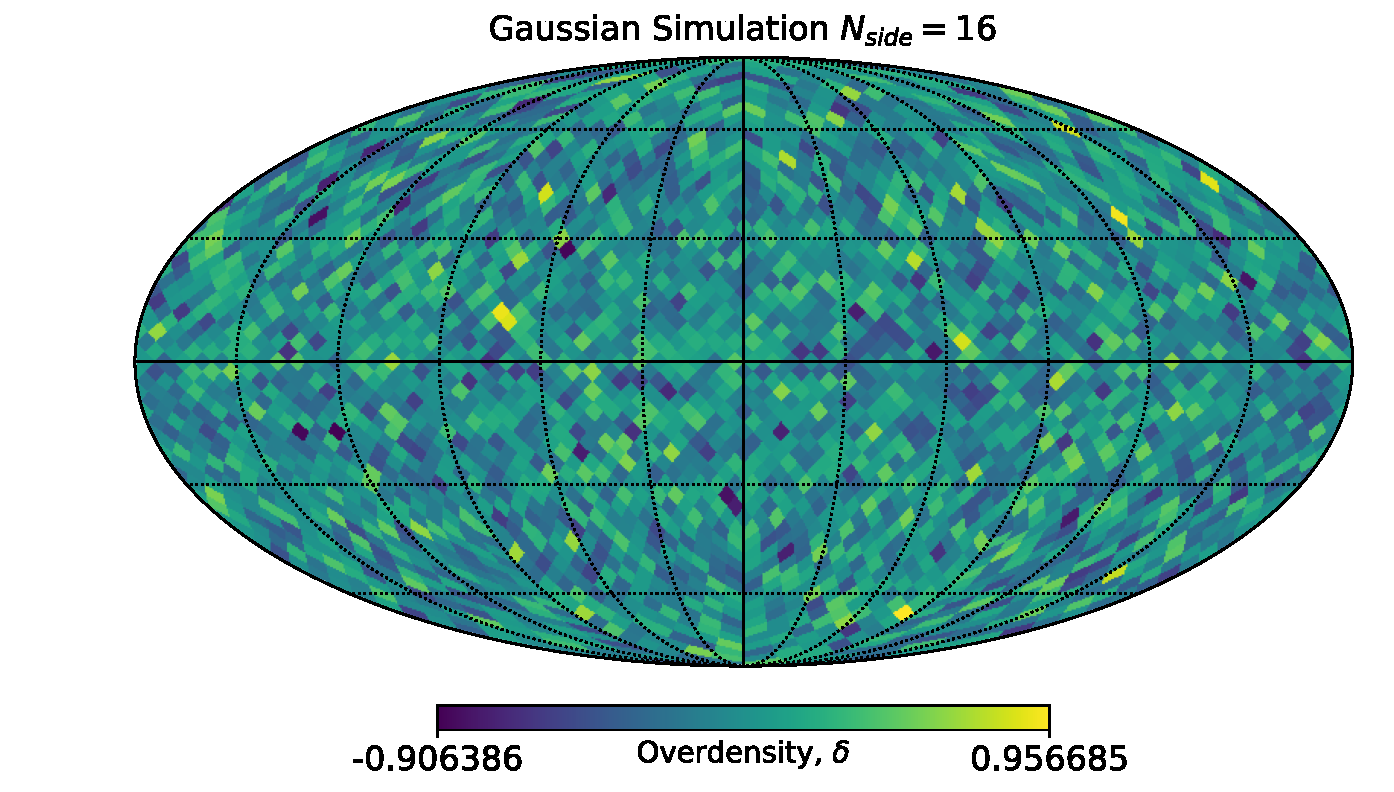
\includegraphics[scale=0.35]{BPL-FIGS/GenData-FullSky-N16_map.pdf}   
  \caption{}
  \label{fig:BPL:GaussFSMAP}
\end{subfigure}\\
\end{center}
\begin{subfigure}{.5\textwidth}
  \centering
  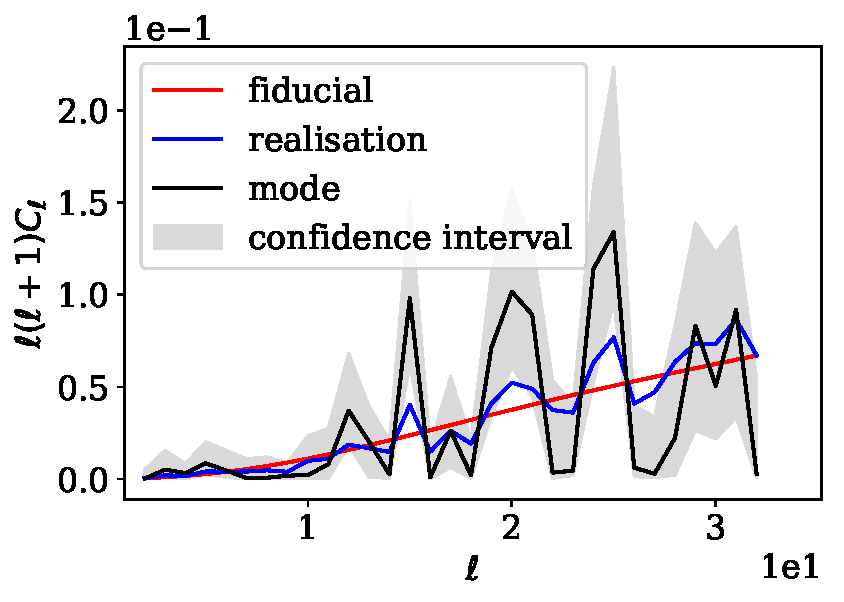
\includegraphics[scale=0.50]{BPL-FIGS/GenData-FullSky-N16clsHPD.pdf}
  \caption{}
\end{subfigure}
\begin{subfigure}{.5\textwidth}
  \centering
  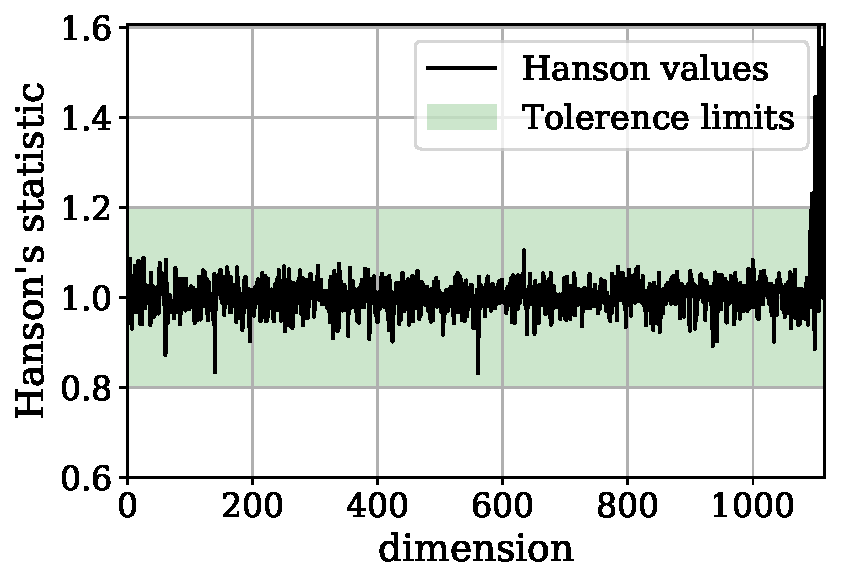
\includegraphics[scale=0.50]{BPL-FIGS/GenData-FullSky-N16_Hanson.pdf}
  \caption{}
\end{subfigure}
\caption[Bayesian-$C_{\ell}$ estimator tested on a full sky Gaussian simulation.]{\textit{(a)} Full sky Gaussian simulation with a Gaussian noise realisation.  \textit{(b)} Results from the Bayesian-$C_{\ell}$ estimator benchmarking tests using Gaussian simulations with Gaussian noise. The red line shows the fiducial angular power spectrum used to generate the simulations, the blue line shows the results obtained with the Pseudo-$C_{\ell}$ estimator, the black line is the mode of the Bayesian estimator samples and the shaded region shows the 68\% confidence regions from the sampled posterior, $\Pr (\{C_{\ell}\}|\mathbf{d})$ \textit{(c)} Convergence diagnosis using the Hanson test on the sampled chain.}% Values between 0.8 and 1.2 demonstrate that an acceptable convergence is able to recover the fiducial power spectrum. Results here were obtained with $N_{samples} = 105,000$.}
\label{fig:BPL:GaussianFSAnalysis}
\end{figure}
This section investigates the behaviour of the Bayesian estimator in the full sky case, comparing the Gaussian and Log-Normal cases. Even thought a full sky case is very far from what one obtains from any type of cosmological survey, it works as a first benchmark test. This methodology has been assessed before for the case of Gaussian simulations in \cite{SreeThesis}; however, the interest in this section is to understand how the method behaves in the Log-Normal case with a Poissonian noise realisation (as described in Section \ref{Sec:BPL:SimData}). Since I am interested in recovering the low-$\ell$ information, I have kept the resolution for these simulations low, with $N_{side} = 16$ (meaning that the sky is then divided into 3072 equal sized pixels). Simulations were both performed using the same fiducial angular power spectra and noise level, with $N^{-1} = \bar{n} = 14.25\,  \text{galaxies}/\text{pixel}$. Figure \ref{fig:BPL:GaussianFSAnalysis} shows the analysis of a Gaussian simulation with Gaussian noise together with the convergence test using the Hanson statistics \footnote{Even though results using this type of simulation were presented previously in the literature, I had added this analysis for completeness and as a sanity check.}. Figure \ref{fig:BPL:LogNormalFSAnalysis} shows the same analysis, now on a Log-Normal simulation with Poissonian noise. Note that, in this case, the noise map used contains anisotropic noise, i. e. it is not constant in the sky. For full sky, using the proper galaxy map as a proxy for the noise does not seem to make an impact; however, as it is shown in Section \ref{Sec:Noise}, it can have a considerable impact for partial sky cases.

\qquad Results from Figures \ref{fig:BPL:GaussianFSAnalysis} and \ref{fig:BPL:LogNormalFSAnalysis} demonstrate that, in a full sky case, the Bayesian-$C_{\ell}$ estimator performs equally well, achieving a satisfactory convergence with a little more than 100,000 samples. The next section looks into the behaviour of low-$\ell$ modes in cases where different masks are applied to the survey.

\begin{figure}
\begin{center}
\begin{subfigure}[b]{.5\textwidth}
 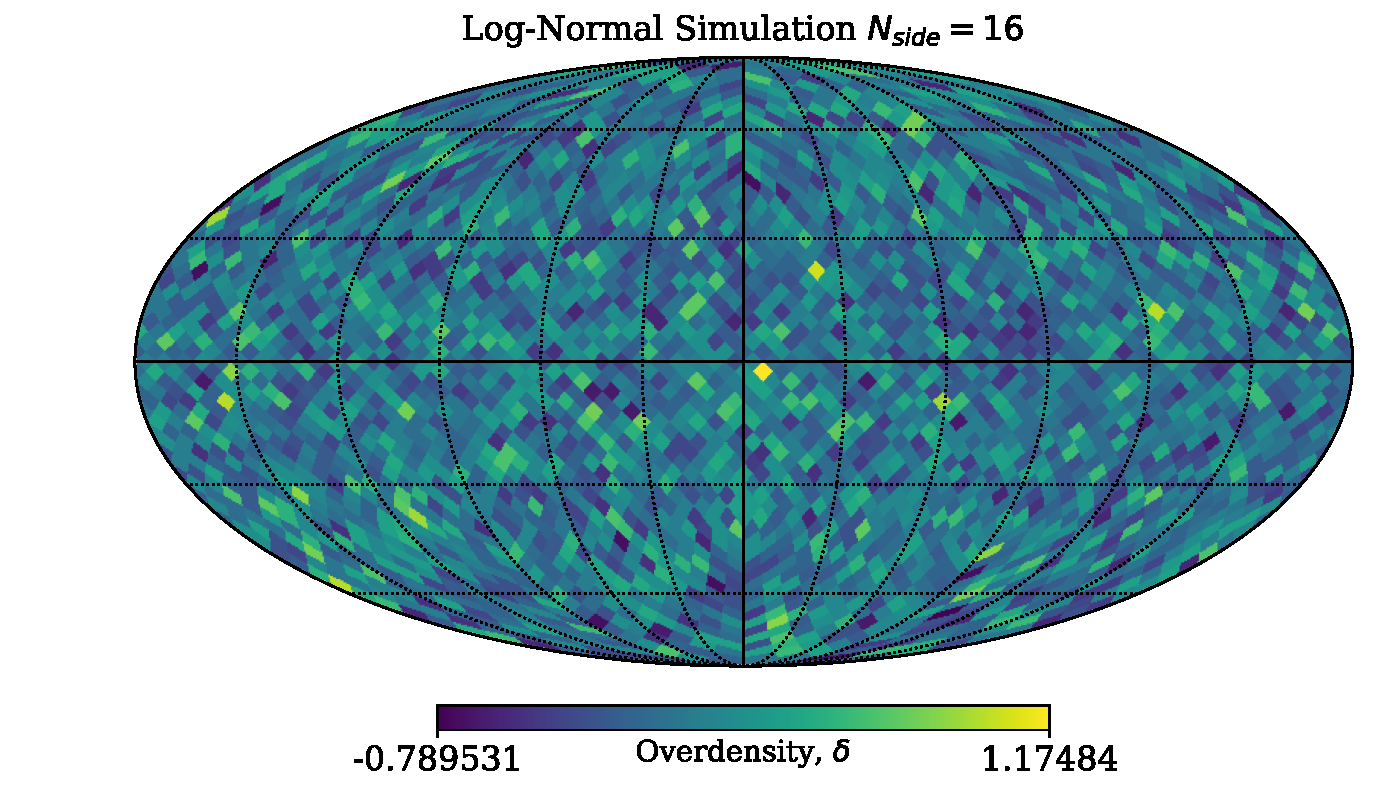
\includegraphics[scale=0.35]{BPL-FIGS/Flask-FullSky-N16_map.pdf}
  \caption{}
  \label{fig:BPL:LNFSMAP}
\end{subfigure}\\
\end{center}
\begin{subfigure}{.5\textwidth}
  \centering
  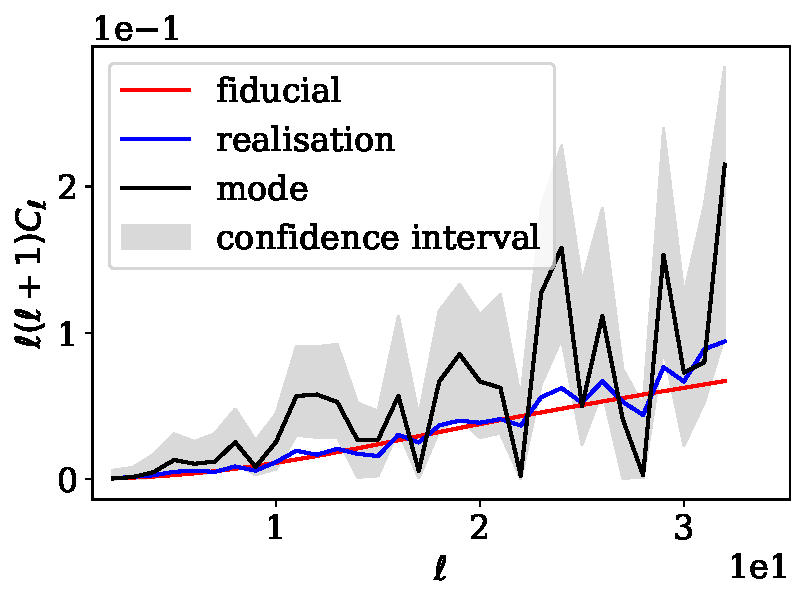
\includegraphics[scale=0.50]{BPL-FIGS/Flask-FullSky-N16clsHPD.pdf}
  \caption{}
\end{subfigure}
\begin{subfigure}{.5\textwidth}
  \centering
  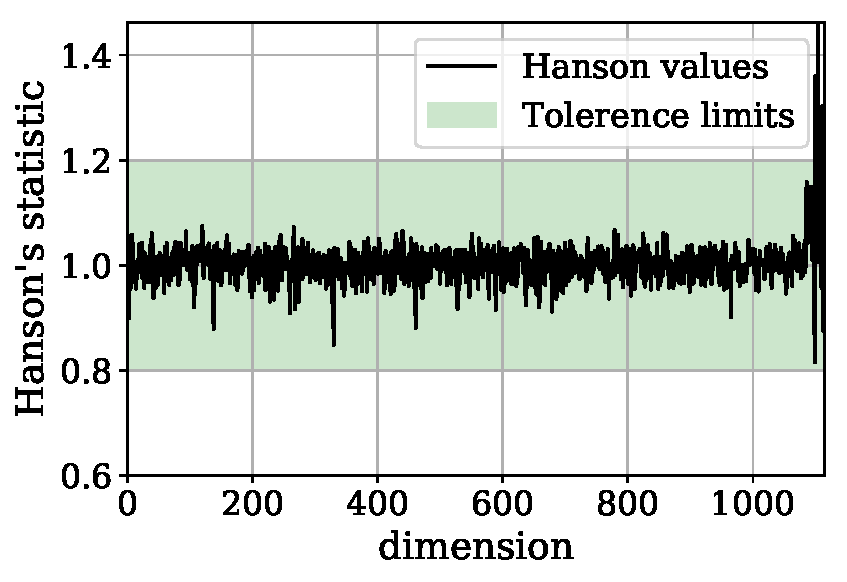
\includegraphics[scale=0.50]{BPL-FIGS/Flask-FullSky-N16_Hanson.pdf}
  \caption{}
\end{subfigure}
\caption[Bayesian-$C_{\ell}$ estimator tested on a full sky \flask log-normal simulation.]{\textit{(a)} Full sky log-normal simulation with a Poissonian noise realisation generated with \flask for galaxy clustering.  \textit{(b)} Results from the Bayesian-$C_{\ell}$ estimator benchmarking tests on a log-normal simulation. The red line shows the fiducial angular power spectrum used to generate the simulation, while the blue line shows the results obtained with the Pseudo-$C_{\ell}$ estimator, and the black line is the mode of the Bayesian estimator samples and the shaded region shows the 68\% confidence regions from the sampled posterior, $\Pr (\{C_{\ell}\}|\mathbf{d})$ \textit{(c)} Convergence diagnosis using the Hanson test on the sampled chain. Values between 0.8 and 1.2 demonstrate that an acceptable convergence is able to recover the fiducial power spectrum. Results here were also obtained with $N_{samples} = 105,000$.}
\label{fig:BPL:LogNormalFSAnalysis}
\end{figure}


\subsection{Investigation of spherical harmonics correlations under a mask}\label{Sec:BPL:AlmsInvestigation}
The presence of a mask in a survey, although realistic, creates correlations between different modes in the $C_{\ell}$s and also in the spherical harmonic coefficients modes and phases. Consider, once more, the spherical harmonic decomposition of a galaxy map,\footnote{A catalogue of galaxies projected in a spherical shell.} $\delta^g$, in a case of partial sky. As in Equation \eqref{Eq:define_delta_p},
\begin{equation}
    \tilde{a}_{\ell m} = \sum_i \delta^p_i Y_{\ell m}(\Omega_i)w_i\Delta\Omega
\end{equation}
where, $\Delta\Omega$ is the area of a pixel in the pixelised map; and $w_i$ is a weight function value at pixel $i$ which can be transformed via spherical harmonic decomposition as \citep{Efstat2004},
\begin{equation}
    \tilde{w}_{\ell m} = \sum w_i Y_{\ell m}(\Omega_i)\Delta\Omega.
\end{equation}
Therefore, according to \cite{PolSpice2001} and \cite{Efstat2004}, the true $a_{\ell m}$, the spherical harmonics if one had a full sky observation, are related to the observed ones as,
\begin{equation}
    \tilde{a}_{\ell m} = \sum_{\ell' m'} a_{\ell' m'}\mathcal{K}_{\ell m \ell' m'}, 
\end{equation}
where the coupling matrix, $\mathcal{K}_{\ell m \ell' m'}$, is defined in terms of the Wigner-3j symbols as
\begin{align}
\label{Eq:Klmlm}
    \mathcal{K}_{\ell m \ell' m'} = & \sum_{\ell'' m''} (-1)^{m'}(-1)^{m''} \tilde{w}_{\ell'' m''} \left[\frac{(2\ell + 1)(2\ell'+1)(2\ell''+1)}{4\pi} \right]^{1/2} \nonumber \\
    & \quad \times \begin{pmatrix} \ell & \ell' & \ell'' \\ 0 & 0 & 0 \end{pmatrix}\begin{pmatrix} \ell & \ell' & \ell'' \\ m & -m' & -m'' \end{pmatrix}.
\end{align}
which accounts for the mixing of modes in the spherical harmonic coefficients in the presence of a mask. This coupling matrix manifest itself as correlations between different $\tilde{a}_{\ell m}$ which are intimately related to the geometry of the survey as the next examples will demonstrate.

\begin{figure}
\begin{subfigure}[b]{.5\textwidth}
 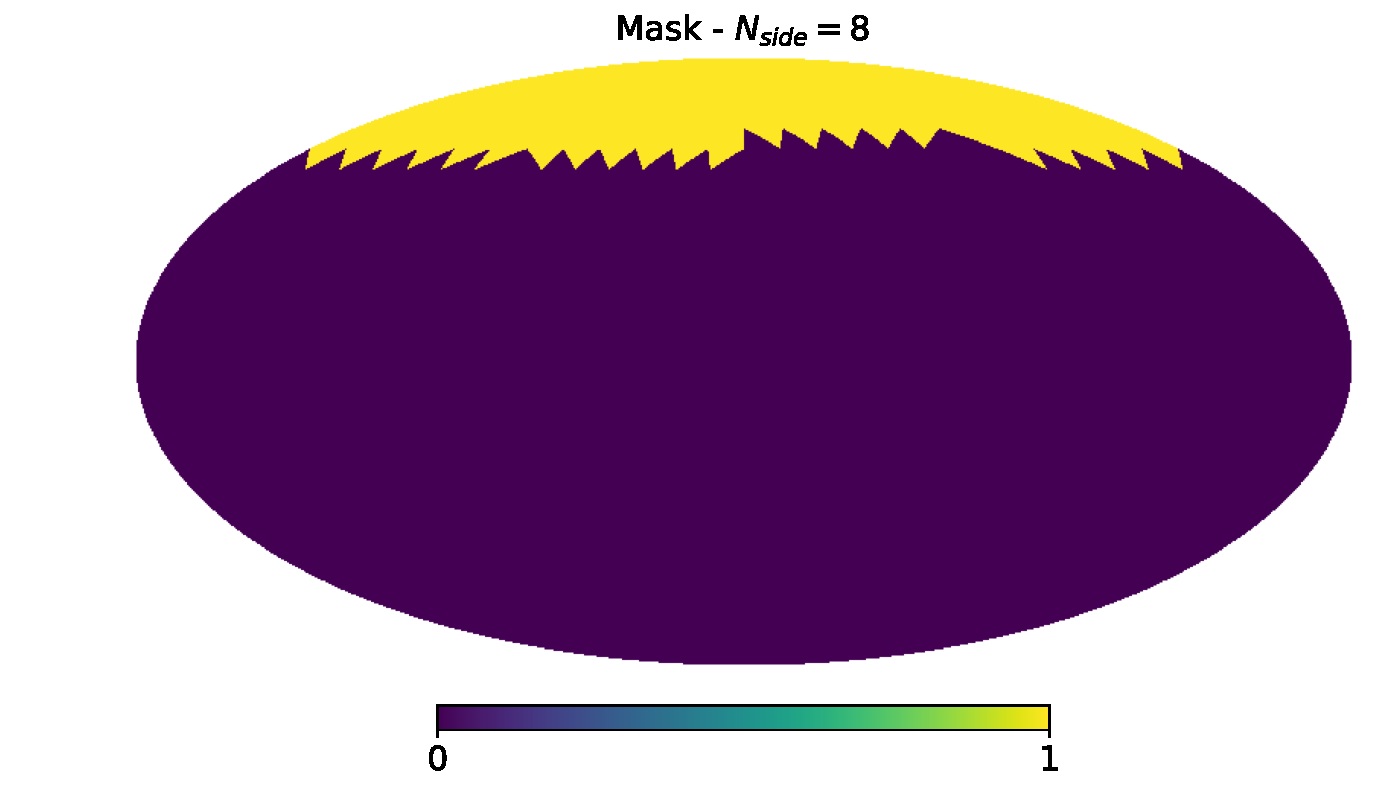
\includegraphics[scale=0.33]{BPL-FIGS/RandomBand_fsky_mask.pdf}
  \caption{Mask with $f_{sky} = 0.1$.}
  \label{fig:BPL:PoleMask}
\end{subfigure}
\begin{subfigure}[b]{.5\textwidth}
 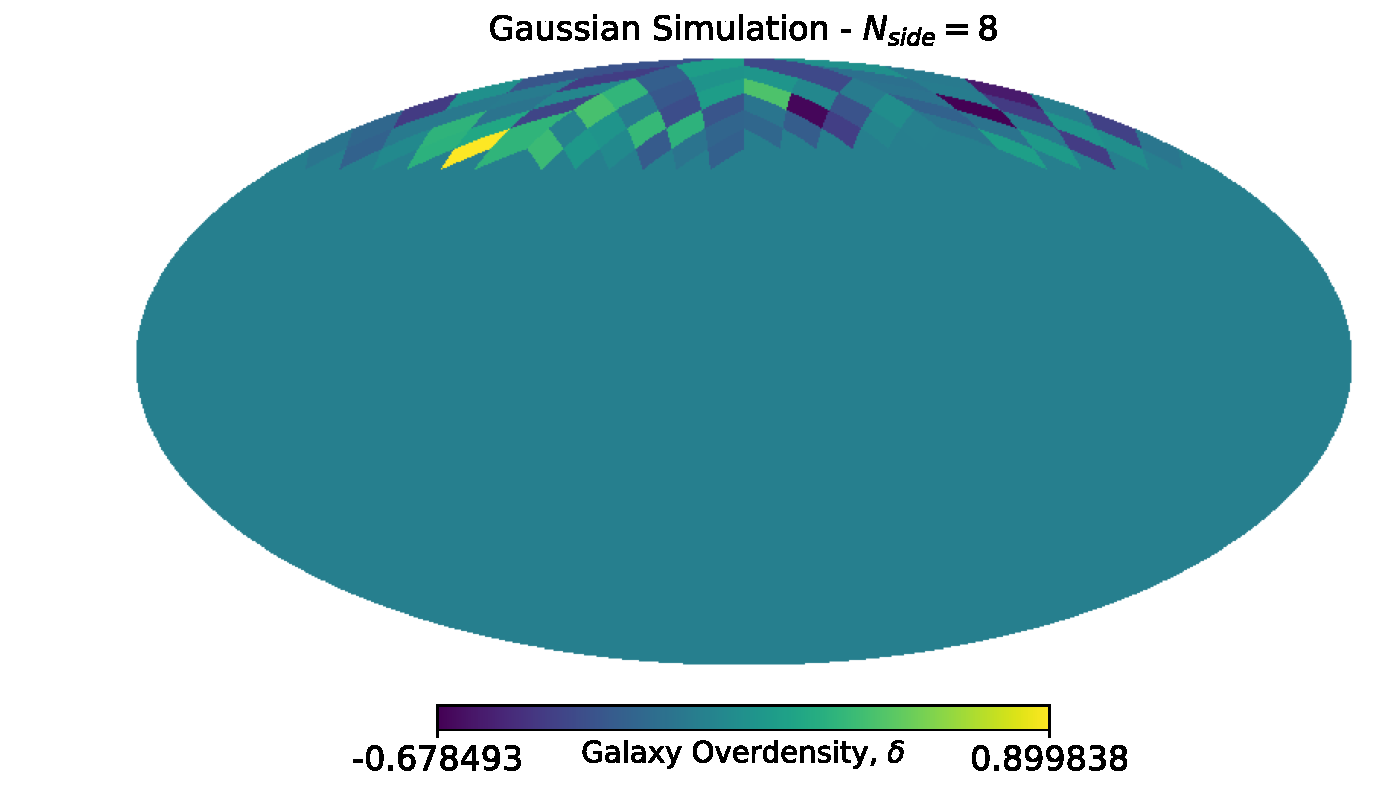
\includegraphics[scale=0.34]{BPL-FIGS/RandomBand_fsky_map.pdf}
  \caption{Simulated data}
  \label{fig:BPL:PoleMap}
\end{subfigure}\\
\begin{subfigure}[b]{\textwidth}
 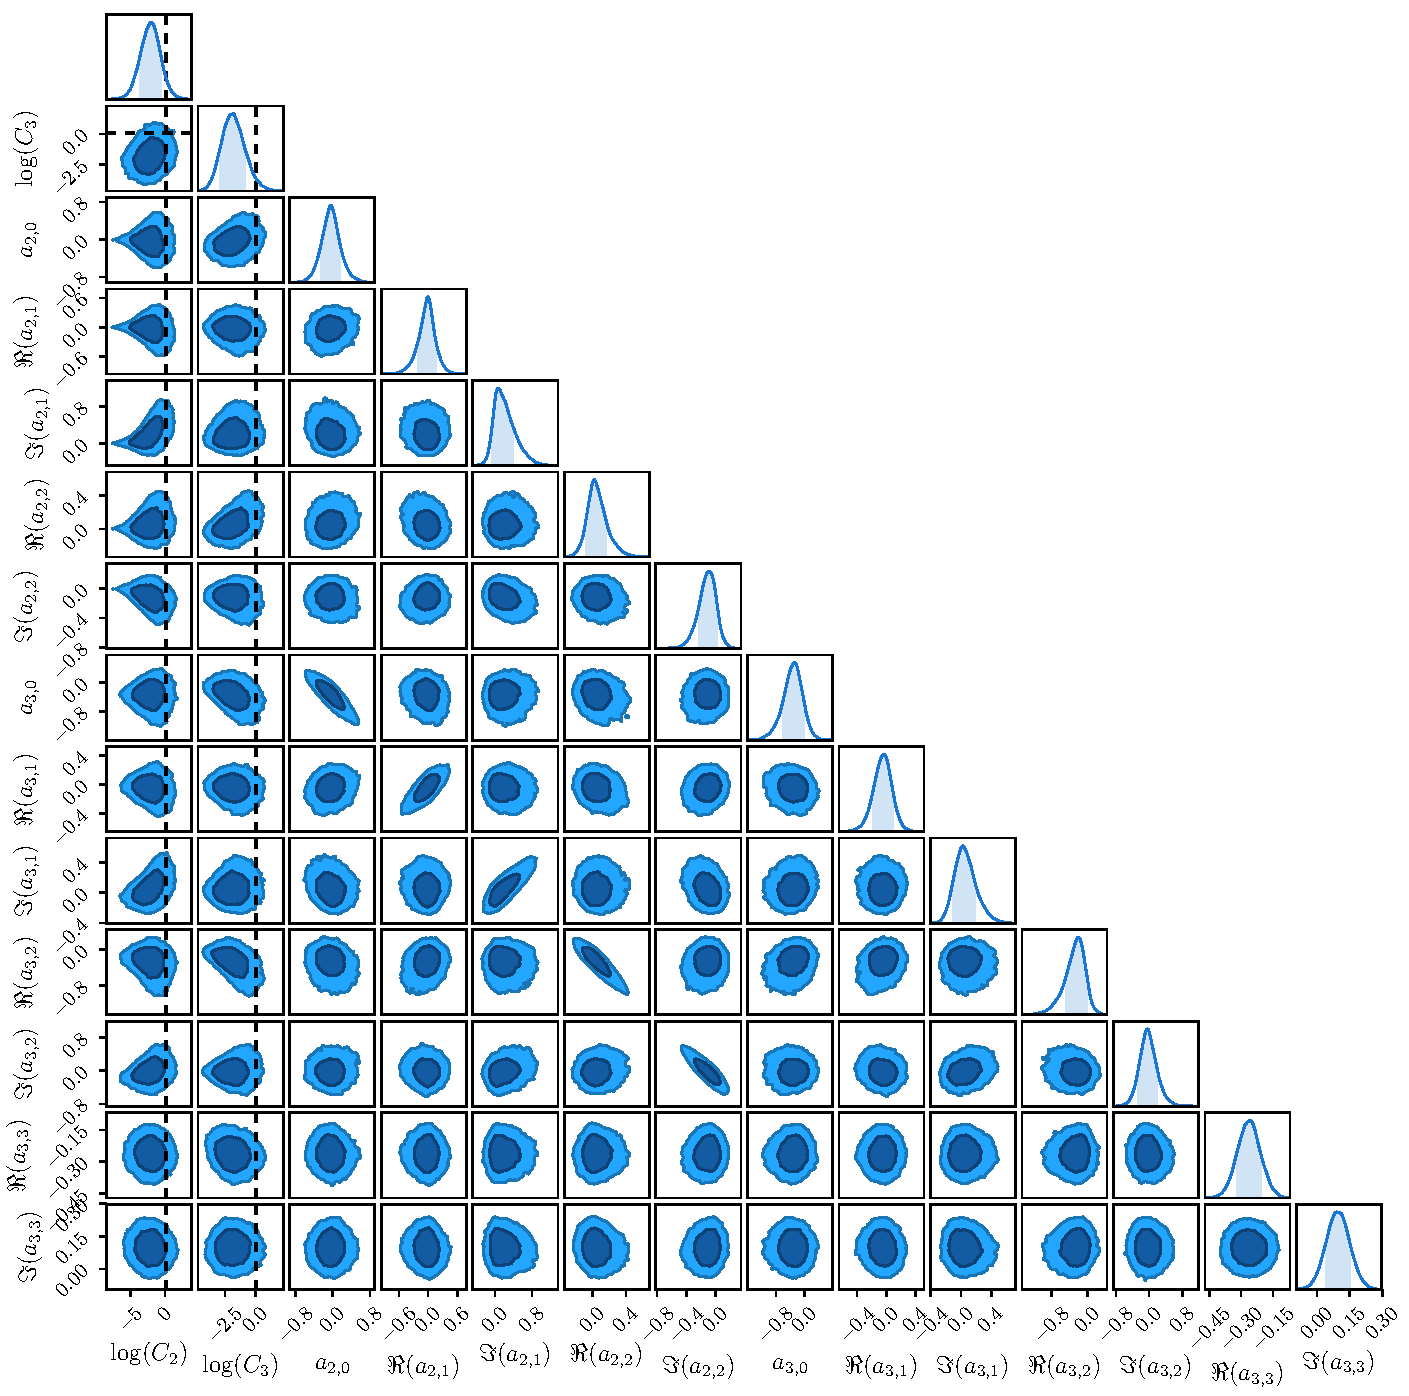
\includegraphics[width=\textwidth]{BPL-FIGS/RandomBand_fsky_01_trianglePlot.pdf}
  \caption{Marginalised posterior}
  \label{fig:BPL:PoleTri}
\end{subfigure}
\caption[Investigation of correlation spherical harmonics for $\ell = 2\, \& \, 3$ for a mask with a spherical cap containing only a 10\% sky fraction]{Investigation of correlations in the spherical harmonics for $\ell = 2\, \& \, 3$ for a mask with a spherical cap containing only a 10\% sky fraction. \textit{(a)} Shows the mask used in the analysis. \textit{(b)} Shows the Gaussian simulated data. Data was generated using only the same modes as the ones probed, $\ell = 2,3$. \textit{(c)} Shows the full posterior for this case, the first two parameters are the $C_{\ell}$s while the following ones are the real and imaginary parts of the related spherical harmonics. Dashed lines show the fiducial $C_{\ell}$ values used to generate the simulations. Note that, in this case, correlations are introduced in $a_{\ell m}$ with the same phase, e.g. same $m$.}
\label{fig:BPL:Pole}
\end{figure}

\qquad Observing only the first two modes, i. e. $\ell = 2 \, \& \, 3$, I investigate here the correlations that are introduced given different considered geometries for the angular selection of a survey. The first two simulations, presented in Figures \ref{fig:BPL:Pole} and \ref{fig:BPL:Blob}, are Gaussian while the one presented in Figure \ref{fig:BPL:Euclid-N8} is Log-Normal. All simulations presented in this section use the same fiducial $C_{\ell}$, noise level, and have a very low-resolution, $N_{side}=8$, as the intention here is \textbf{not} to marginalise over the spherical harmonic coefficients. Even thought the intention of this section is merely illustrative, going to higher resolutions and higher modes without treating the $a_{\ell m}$ as nuisance parameters requires a great amount of computational disk space and also impractical to observe correlations between the coefficients. 

\qquad The first first mask, presented in Figure \ref{fig:BPL:PoleMask} is a spherical cap in the northern galactic pole with observations covering around 10\% of the sky; the mask, overdensity map (generated from a Gaussian simulation), and marginalised 1 and 2D posteriors for $C_{\ell}$s and $a_{\ell m}$ are presented in Figure \ref{fig:BPL:Pole}. By analysing the triangle plot presented in Figure \ref{fig:BPL:PoleTri}, correlations between spherical harmonic coefficients appear (as predicted by Equation \ref{Eq:Klmlm}). For this specific mask, due to its asymmetric nature, the correlations are introduced in spherical harmonic coefficients with different $\ell$-modes but different phases, i. e. $a_{\ell m}$ with $a'_{\ell' m}$. These degeneracies cause the deviation observed in the 1D marginalised posterior for the $C_{\ell}$s (the first two columns in Figure \ref{fig:BPL:PoleTri}).

\qquad The second example case analysed in this section is a mask with four different size caps, placed symmetrically in the sphere. This mask, presented in Figure \ref{fig:BPL:blobMask}, contains around 31\% of sky coverage. The mask, Gaussian simulation of an overdensity field, and the marginalised posteriors for this case are presented in Figure \ref{fig:BPL:Blob}. Observing the correlation between $a_{\ell m}$ in the posteriors, one can see that it is different from the previous case presented in Figure \ref{fig:BPL:PoleTri}: correlations now are between spherical harmonic coefficients with different modes and phases. As expected, this is due to the geometry of the mask which presents different sized caps -- explaining why correlation with different $\ell$-modes -- and caps situated in symmetrical regions on the sphere -- correlating the phases too. In other words, the analysed geometry correlates $a_{\ell m}$ and $a'_{(\ell-1),(m-1)}$; yet, the angular power spectra suffers no biases due to these correlations as it can be seen from the first two columns in Figure \ref{fig:BPL:BlobTriang}.

\begin{figure}
\begin{subfigure}[b]{.5\textwidth}
 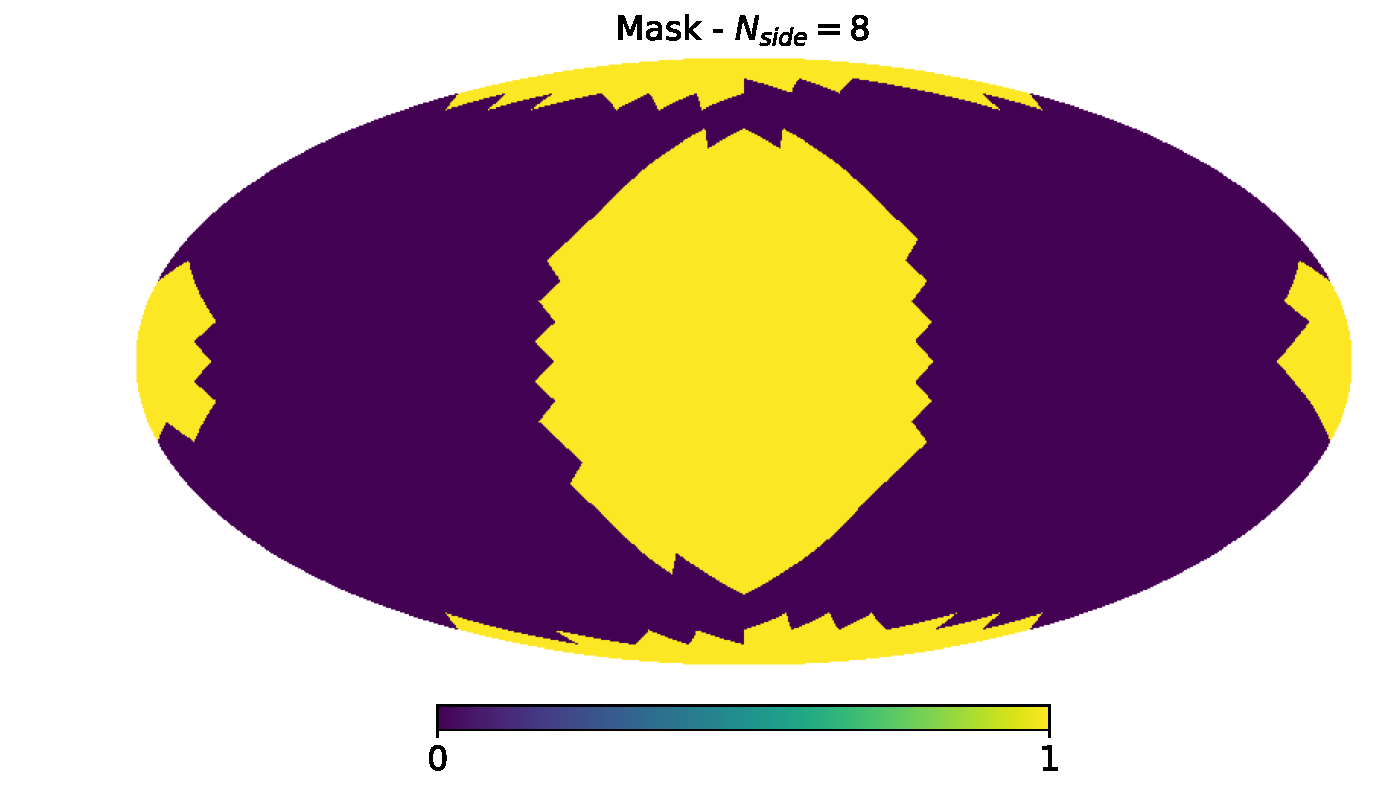
\includegraphics[scale=0.33]{BPL-FIGS/Blob_fsky_01_mask.pdf}
  \caption{Mask with $f_{sky} \approx 0.31$.}
  \label{fig:BPL:blobMask}
\end{subfigure}
\begin{subfigure}[b]{.5\textwidth}
 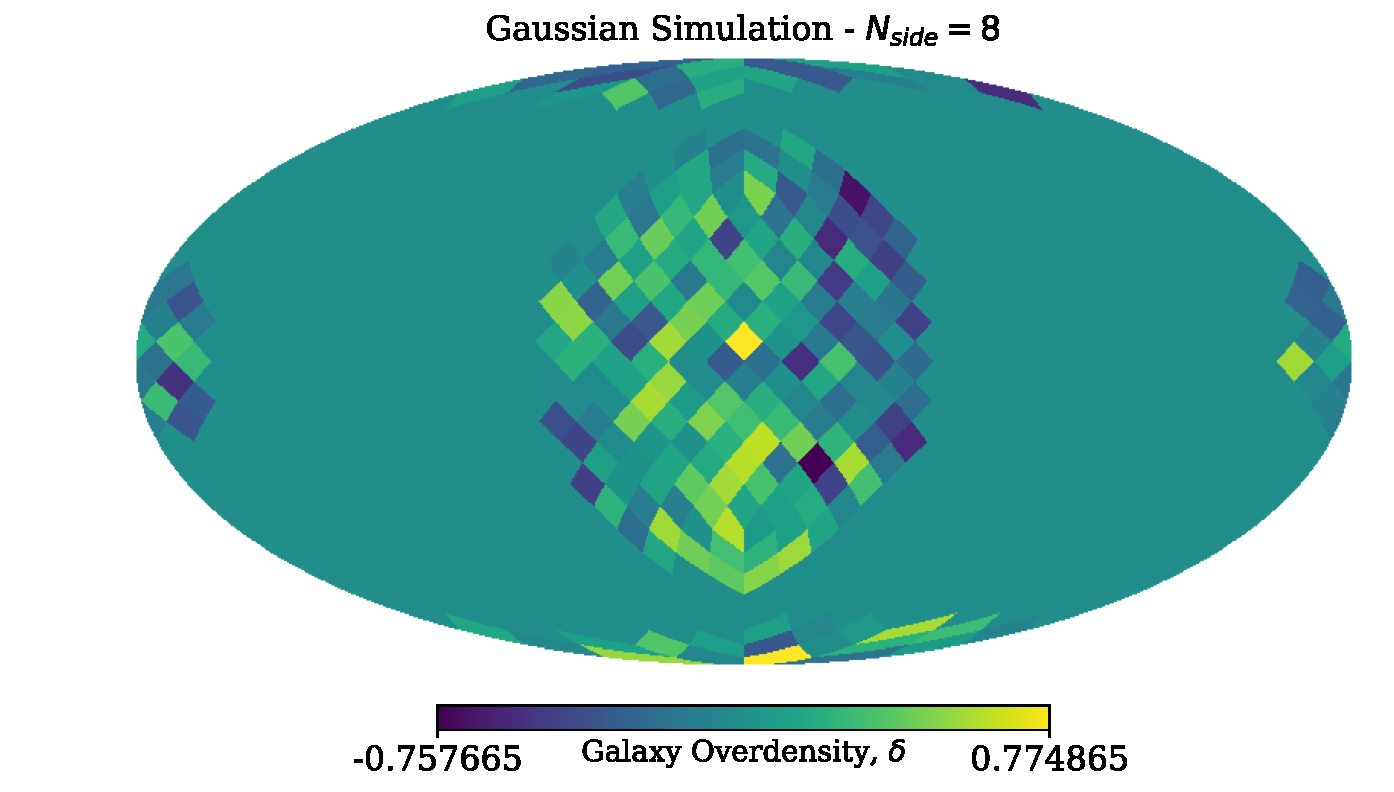
\includegraphics[scale=0.34]{BPL-FIGS/Blob_fsky_01_map.pdf}
  \caption{Simulated data}
  \label{fig:BPL:blobMap}
\end{subfigure}\\
\begin{subfigure}[b]{\textwidth}
 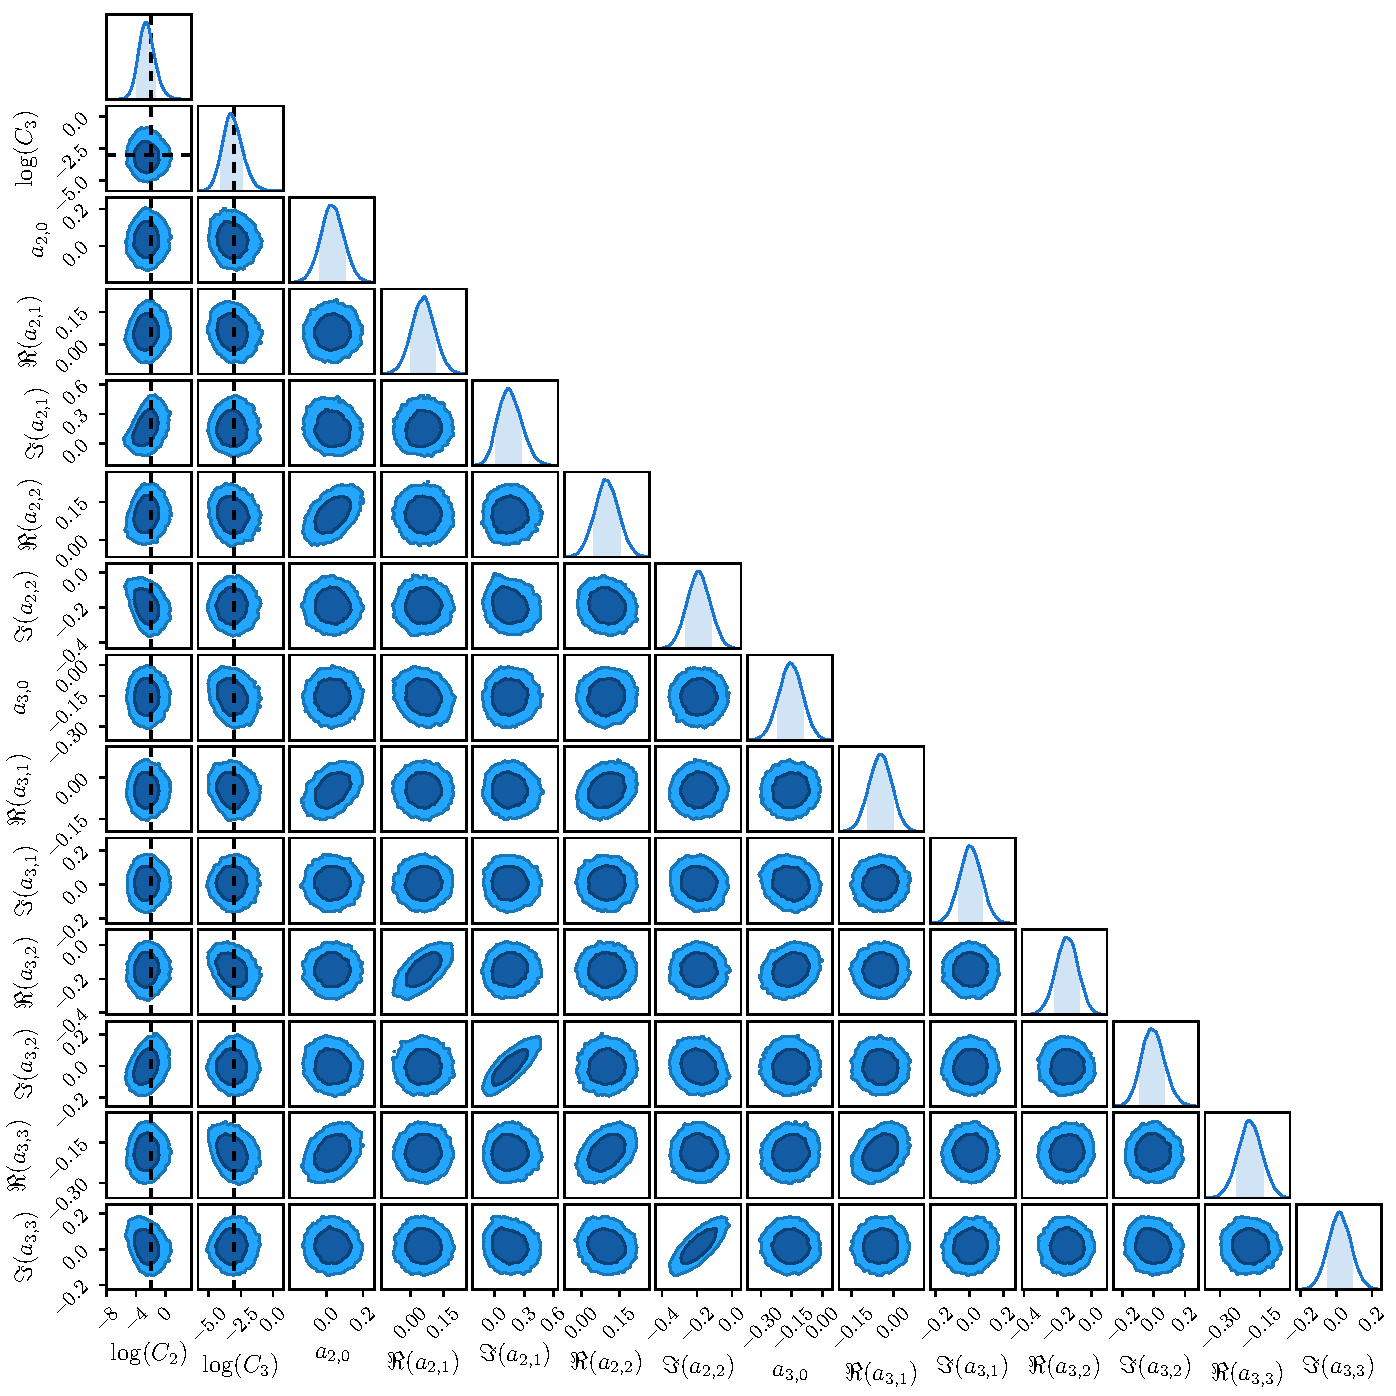
\includegraphics[width=\textwidth]{BPL-FIGS/Blob_fsky_01_trianglePlot.pdf}
  \caption{Marginalised posterior}
  \label{fig:BPL:BlobTriang}
\end{subfigure}
\caption[Investigation of correlation spherical harmonics for $\ell = 2\, \& \, 3$ for a mask with four spherical caps with different sizes containing a 10\% sky fraction]{Investigation of correlations in the spherical harmonics for $\ell = 2\, \& \, 3$ for a mask with four spherical caps with different sizes. This simulation contains 31\% sky coverage. \textit{(a)} Shows the mask used in the analysis. \textit{(b)} Shows the Gaussian simulated data. Data was generated using only the same modes as the ones probed, $\ell = 2,3$. \textit{(c)} The full posterior for this case, the first two parameters are the $C_{\ell}$s while the following ones are the real and imaginary parts of the related spherical harmonics. Dashed lines show the fiducial $C_{\ell}$ values used to generate the simulations. For this survey geometry, correlations are introduced between $a_{\ell m}$ and $a'_{(\ell-1),(m-1)}$. However, such correlations do not deviate the marginalised posterior on the $C_{\ell}$s from the fiducial value.}
\label{fig:BPL:Blob}
\end{figure}

\qquad For the final example in this section, I have analysed a low resolution Euclid-like mask. For this analysis, I used a \flask log-normal simulation with Poissonian noise reflecting the forecasts for the Euclid redshift distribution presented in \cite{2011EuclidRedPaper}. The objective here was to perform an investigation of the possible impact of the Euclid survey strategy in low-$\ell$ modes. Figure \ref{fig:BPL:Euclid-N8} shows the low-resolution Euclid-like mask, the overdensity field sampled from a log-normal simulation with a Poissonian realisation to obtain poin-like sources (as explained in Section \ref{Sec:BPL:SimData}), and the marginalised posteriors for the low-$\ell$ power spectra and spherical harmonic coefficients. For this case, as expected due to the complex geometry of the mask, the correlation do not follow a simple and predictable trend as the previous two cases. Instead, some weak correlations and anti-correlations appear in different combinations of scales and phases. Note that this reflects in the $C_{\ell}$s as a small bias between the sampled values and the fiducial value used to generate the simulation.

\qquad The investigation in this Section demonstrated that some geometries can introduce a small bias in the estimated $C_{\ell}$s for some survey geometries, in the low-$\ell$ regime. Even though some intuition was gained about the impact of the survey's angular geometry in the sampled $a_{\ell m}$ and their correlations, it is not trivial to tell which correlations can and cannot introduced a bias in the marginalised angular power spectra. It is clear from this investigation that the treatment of the principal coordinates of the Hessian as being just their diagonal (see Section \ref{Sec:BPL:Hessian}) leads an incorrect performance of the algorithm when strong correlations appear. A future implementation of the full Hessian calculation for low-$\ell$ modes, in the $C_{\ell}$ space as much as in the $a_{\ell m}$ space, could improve this issue.


%This correlations introduced by the mask in the $a_{\ell}m$s coefficients can be explained via the coupling matrix above \RED{find that paper tomorrow and put the thing here}:



\begin{figure}
\begin{subfigure}[b]{.5\textwidth}
 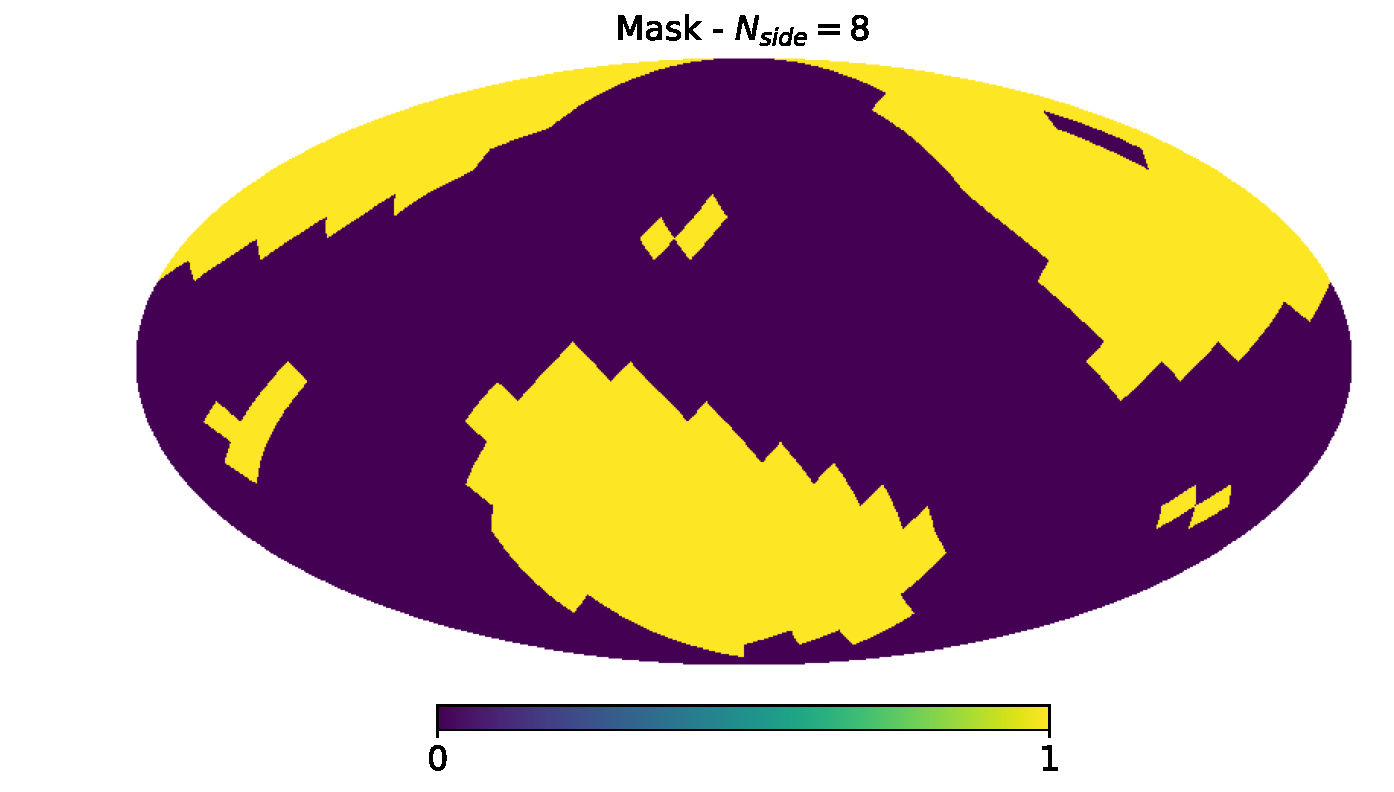
\includegraphics[scale=0.33]{BPL-FIGS/Flask-Euclid-lowEll-N8_mask.pdf}
  \caption{Euclid-Like Mask with $f_{sky} = 0.336 $.}
  \label{fig:BPL:LN-Euclid-N8-mask}
\end{subfigure}
\begin{subfigure}[b]{.5\textwidth}
 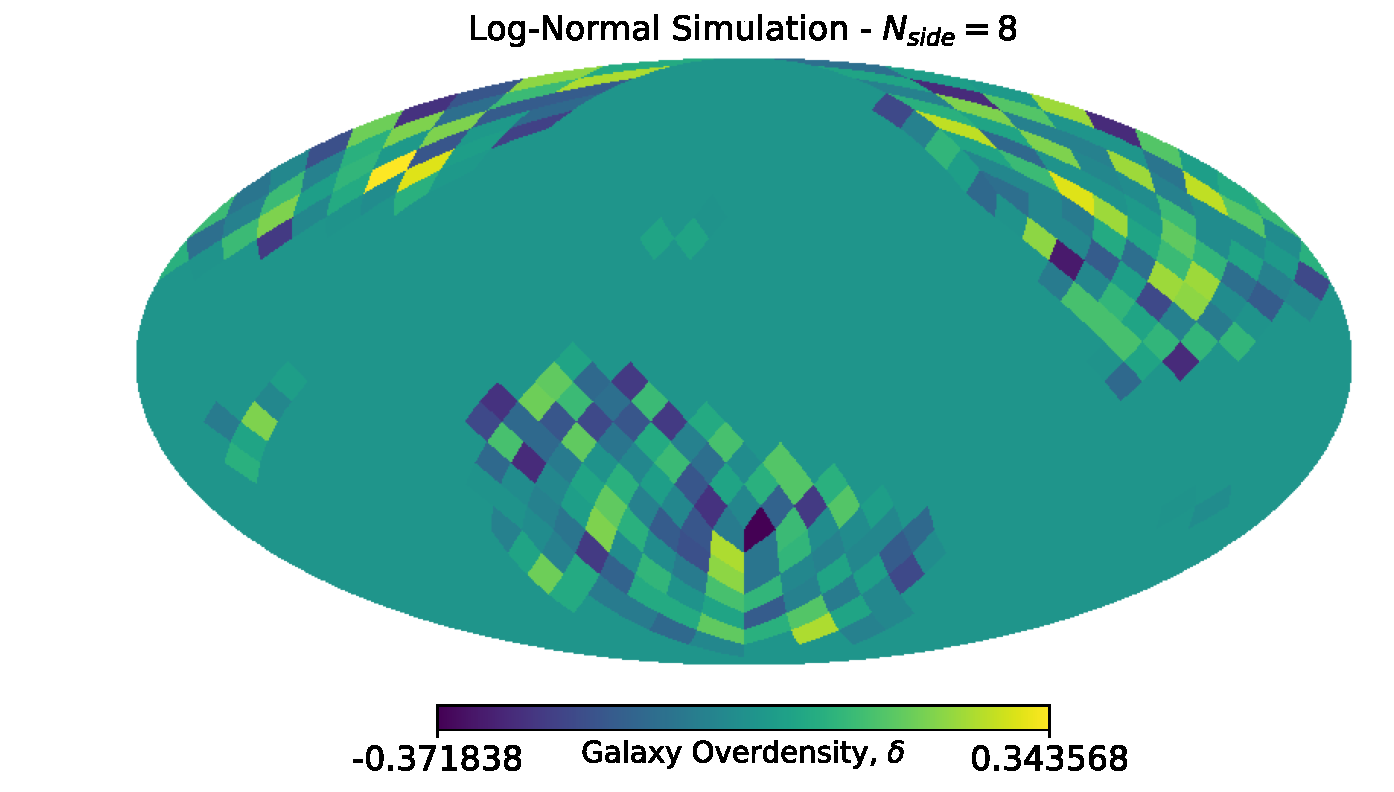
\includegraphics[scale=0.34]{BPL-FIGS/Flask-Euclid-lowEll-N8_map.pdf}
  \caption{Simulated data}
  \label{fig:BPL:LN-Euclid-N8-dens}
\end{subfigure}\\
\begin{subfigure}[b]{\textwidth}
 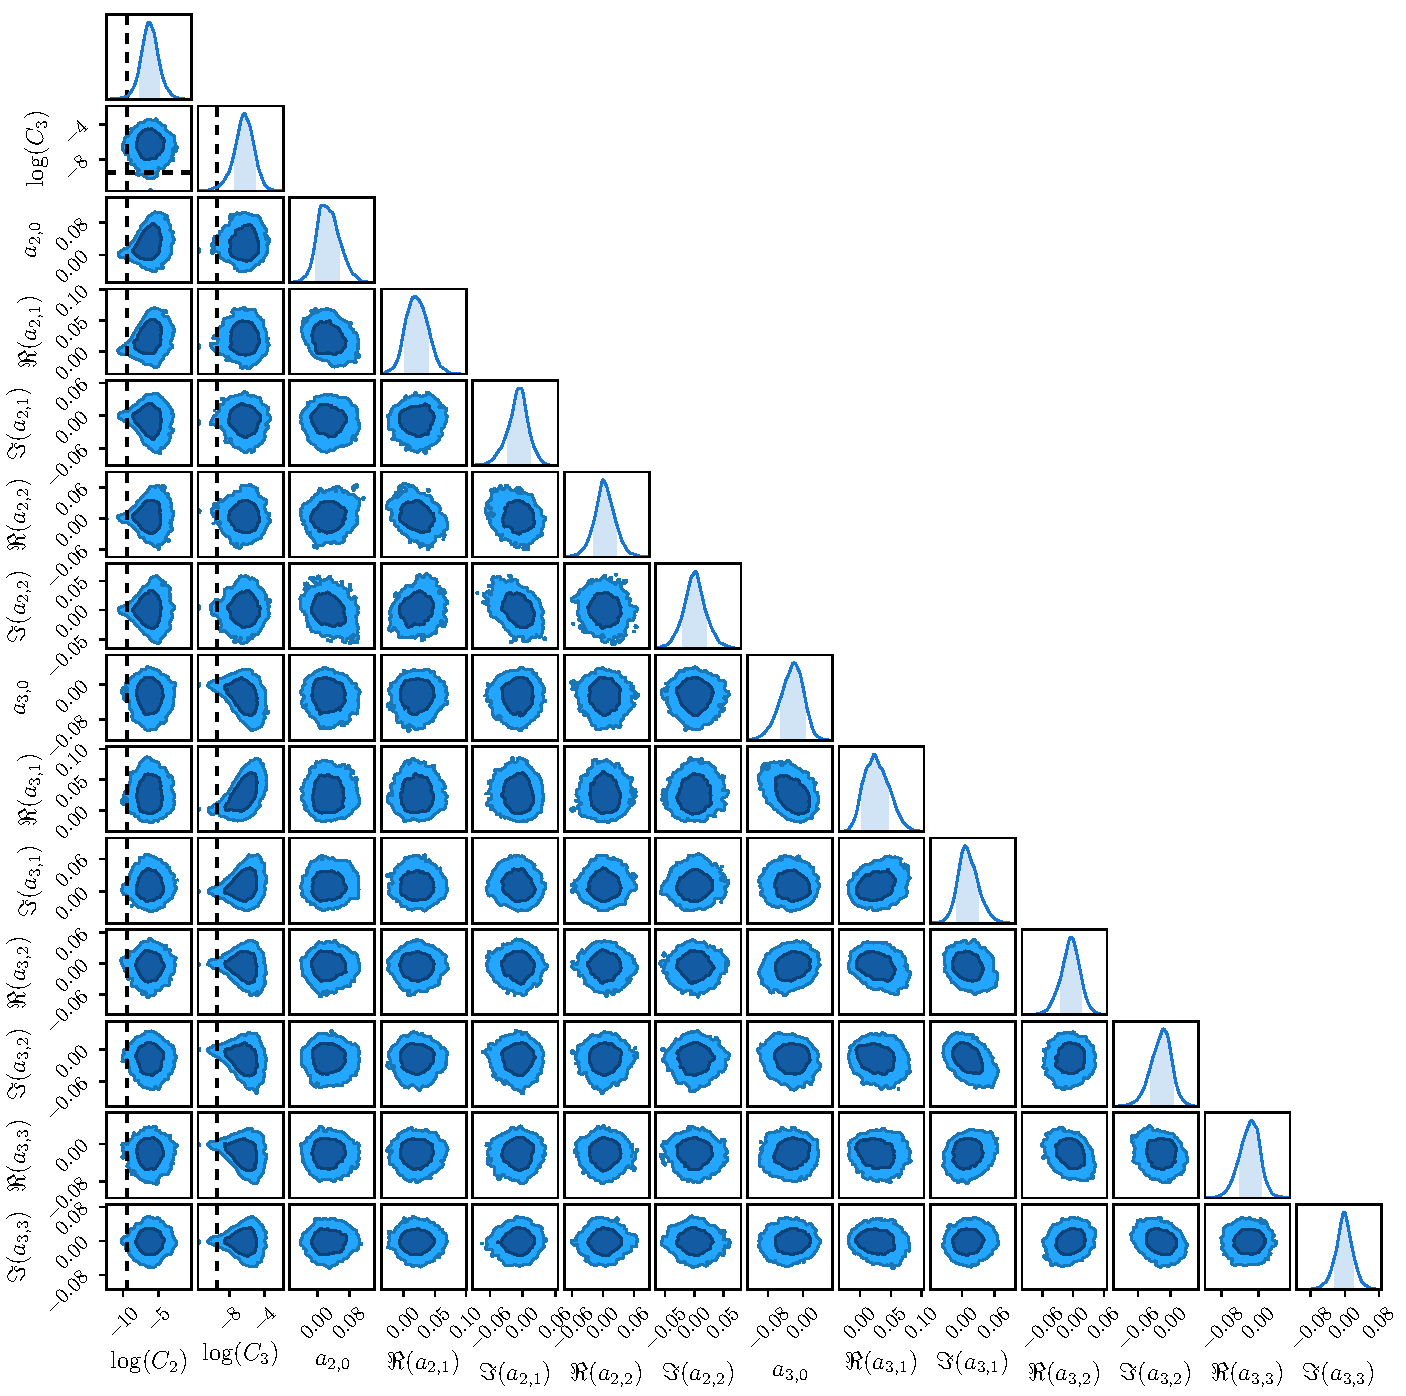
\includegraphics[width=1.05\textwidth]{BPL-FIGS/Flask-Euclid-lowEll-N8_trianglePlot.pdf}
  \caption{Marginalised posterior}
  \label{fig:BPL:LN-Euclid-N8-triang}
\end{subfigure}
\caption[Investigation of correlation in spherical harmonics for $\ell = 2\, \& \, 3$ for a low resolution Euclid-like mask containing a 33.6\% sky fraction]{Correlation between spherical harmonics for $\ell = 2\, \& \, 3$ for a low resolution Euclid-like mask. This simulation contains 33.6\% sky coverage. \textit{(a)} Mask used in the simulation. \textit{(b)} Shows the Log-normal simulated data with Poissonian noise, generated using only $\ell = 2,3$. \textit{(c)} Once more, the full posterior resulting from the Bayesian estimator. First two parameters are the $C_{\ell}$s while the following ones are the real and imaginary parts of the related spherical harmonics. Dashed lines show the fiducial $C_{\ell}$ values used to generate the simulations. This case contains more complex correlations between the $a_{\ell m}$.}
\label{fig:BPL:Euclid-N8}
\end{figure}

\subsection{Anisotropic Noise: Case Study of Euclid's Clustering}\label{Sec:Noise}
In this last investigative Section, I will study the performance of the Bayesian estimator for a more realistic Euclid-like case in a $\ell$-range between $2 \leq \ell \leq 64$. I produced two log-normal simulations with $N_{side}=32$ at a redshift range of $0.5 \leq z < 0.6$ and using the same fiducial $C_{\ell}$ and Euclid-like mask (See Figure \ref{fig:BPL:EuclidMask}). The difference between the two simulations is the signal-to-noise in each one of them -- differing by a factor of $\mathcal{O}(10^4)$. The idea in this section is to investigate how the method outline through this chapter behaves in the presence of two extreme signal-to-noise levels and also to demonstrate that in the case of galaxy clustering, the best proxy for the inverse-noise map is the actual galaxy map, instead of a map where one has the mean number of observed galaxies, $\bar{n}$ (as it is the case for CMB reported by \cite{SreeThesis}). 

\qquad When considering an isotropic noise for galaxy clustering, the Bayesian estimator cannot find the true peak of the Hessian. Instead, it starts sampling so far away from the peak that two possible scenarios happen. The first one is the case where, even though far away from the true peak, the GHS actually finds the peak after a very long burn-in. This is rarely the case. The second, and most common, case is when the sampler gets lost around a local maxima in prior space. It then samples around this maxima without ever finding the true peak of the posterior. This local maxima is usually several orders of magnitude away from the fiducial value, leading to completely incorrect estimation of the power spectrum. I would like to point out here that, when probing a case with full sky, this problem might not appear at first hand; this is mostly due to the fact that for a full sky simulation, the correlations between spherical harmonics do not appear, therefore the noise will be, by construction, isotropic. In the presence of a mask, the anisotropic nature of the Poissonian noise in the galaxy clustering case needs to be dealt with properly for the case of a Bayesian estimator. Therefore, I use here the real galaxy count map as a proxy for the inverse-noise map. Results in this section demonstrate that this is the optimal way to deal with this issue.

\begin{figure}
\begin{center}
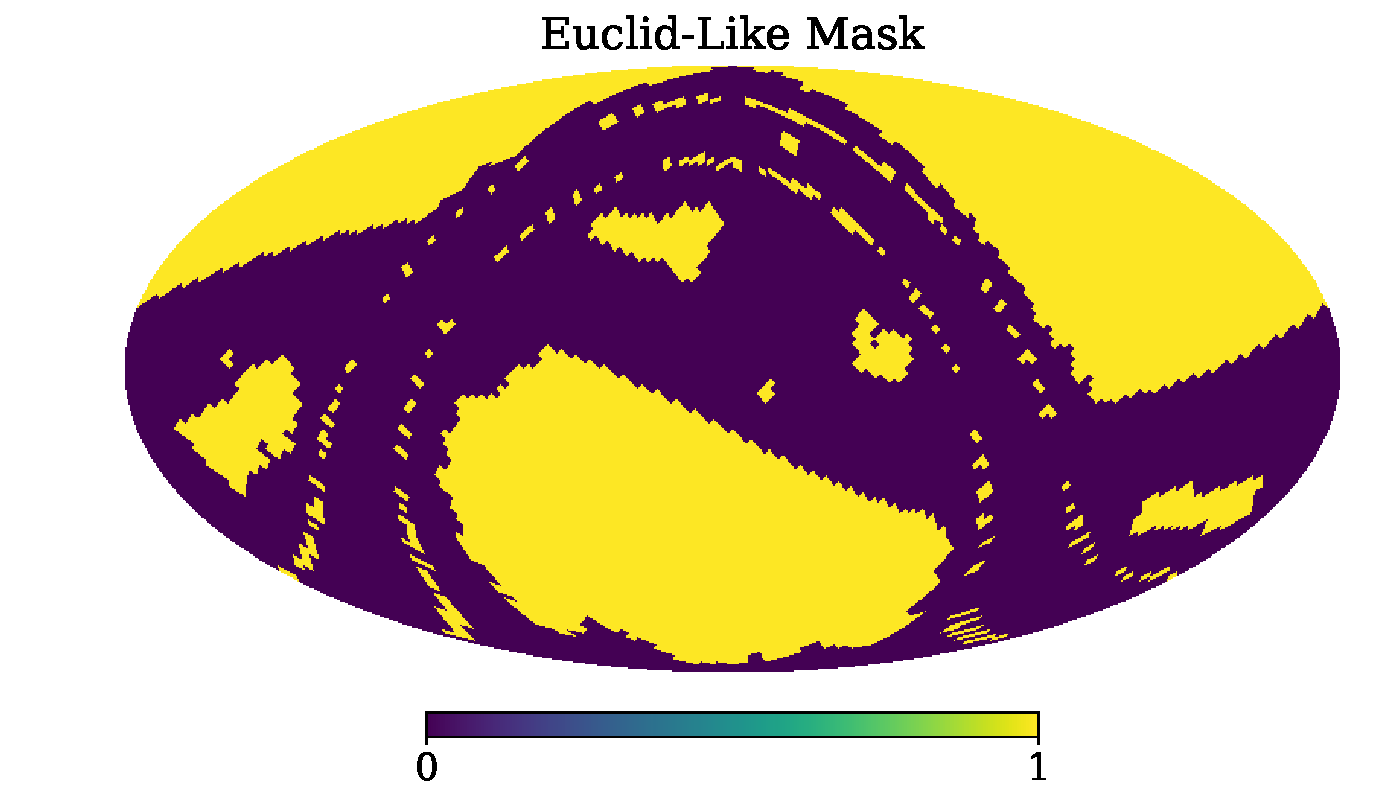
\includegraphics[scale=0.40]{BPL-FIGS/Euclid-Foot-N32.pdf}
\caption[Euclid-like mask with $N_{side} = 32$]{Euclid-like mask with $N_{side} = 32$ used for the simulations and analysis presented in Figures \ref{fig:BPL:LogNormalFSAnalysis} and \ref{fig:BPL:LogNormalFSAnalysisHighSN}.}
\label{fig:BPL:EuclidMask}
\end{center}
\end{figure}

\qquad For the first simulation, presented in Figure \ref{fig:BPL:LN-LowSN-overd}, the number of galaxies was suppressed by a factor of $10^{-4}$ related to the expected number of galaxies observed by Euclid at the given redshift range \citep{2011EuclidRedPaper}. This results in a mean isotropic noise of $\bar{n}^{-1}\approx 2.85\times 10^{-4}$ steradians/galaxies. Nonetheless, as mentioned in the previous paragraph, I used the number counts galaxy map shown in Figure \ref{fig:BPL:LN-LowSN-noise} as the inverse-noise map for the Bayesian angular power spectrum estimator. Results from the Bayesian estimator are shown in Figure \ref{fig:BPL:LN-LowSN-Cls}. Satisfactory convergence in the was achieved in the chains with 335,000 samples as shown for the Hanson statistics plot in \ref{fig:BPL:LN-LowSN-Hanson}. Even though at first look the marginalised $C_{\ell}$ estimates do not look great when compared to estimates from a Pseudo-$C_{\ell}$ estimator (blue line in Figure \ref{fig:BPL:LN-LowSN-Cls}), when carefully looking to the 1D marginalised posteriors one can see that in most cases the peak of the posterior is close to the fiducial value. 

\qquad Figure \ref{fig:BPL:Euclid-Ells} shows a few examples for the 1D marginalised posterior for some $\ell$-modes. Note that, for some cases, the marginalised posterior demonstrate a local maximum near the region where the Pseudo-$C_{\ell}$ estimate is. However, the last panel in Figure \ref{fig:BPL:Euclid-Ells} exhibits a very prominent secondary peak which could be an artefact of the chain not being fully converged in that specific dimension -- note the high values in the last dimensions in Figure \ref{fig:BPL:LN-LowSN-Hanson}. Although, a similar behaviour was present when the chain had 100,000 less samples and did not go away, leading me to believe the amount of samples necessary to converge this part of the chain was higher than I expected.

\begin{figure}
\begin{subfigure}[b]{.5\textwidth}
 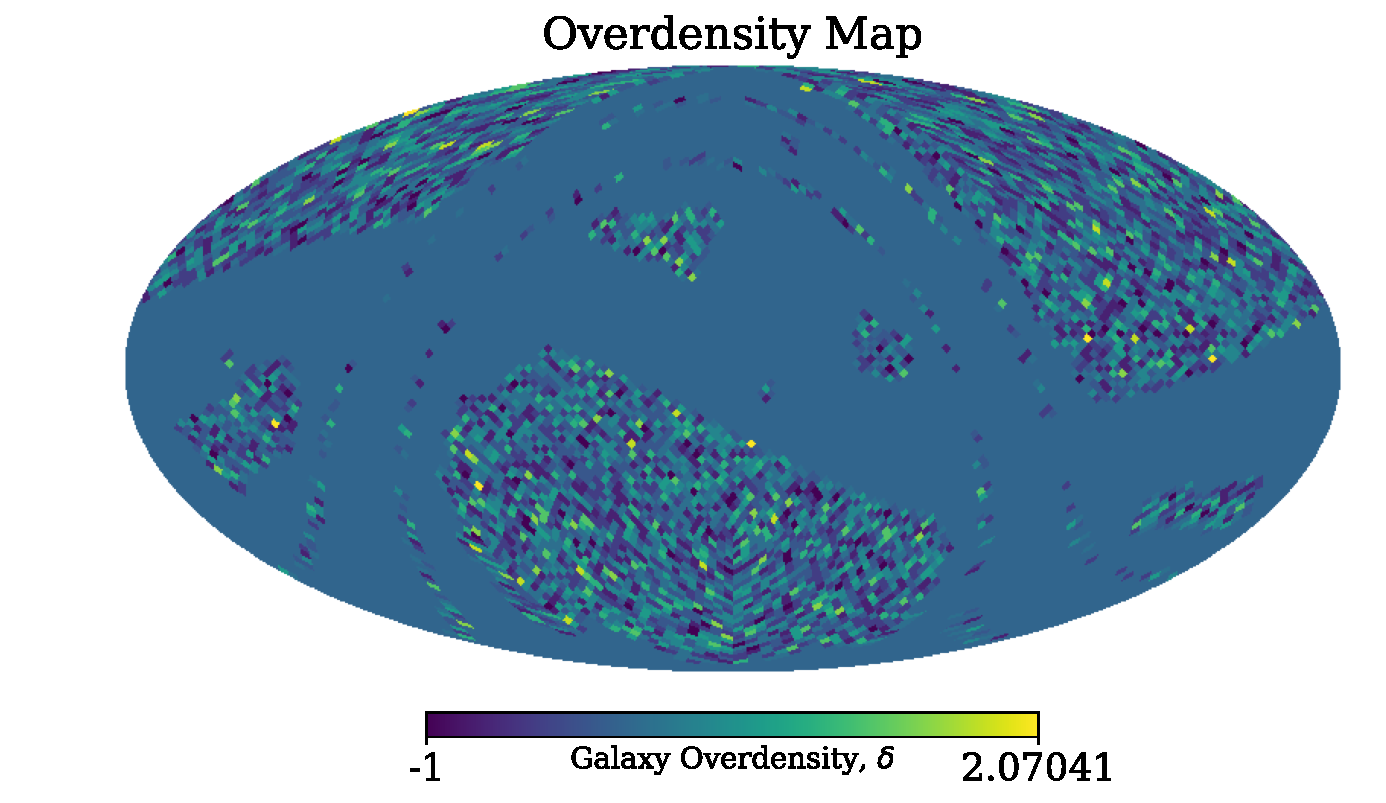
\includegraphics[scale=0.35]{BPL-FIGS/Euclid-Overdensity-N32.pdf}
  \caption{}
  \label{fig:BPL:LN-LowSN-overd}
\end{subfigure}
\begin{subfigure}[b]{.5\textwidth}
 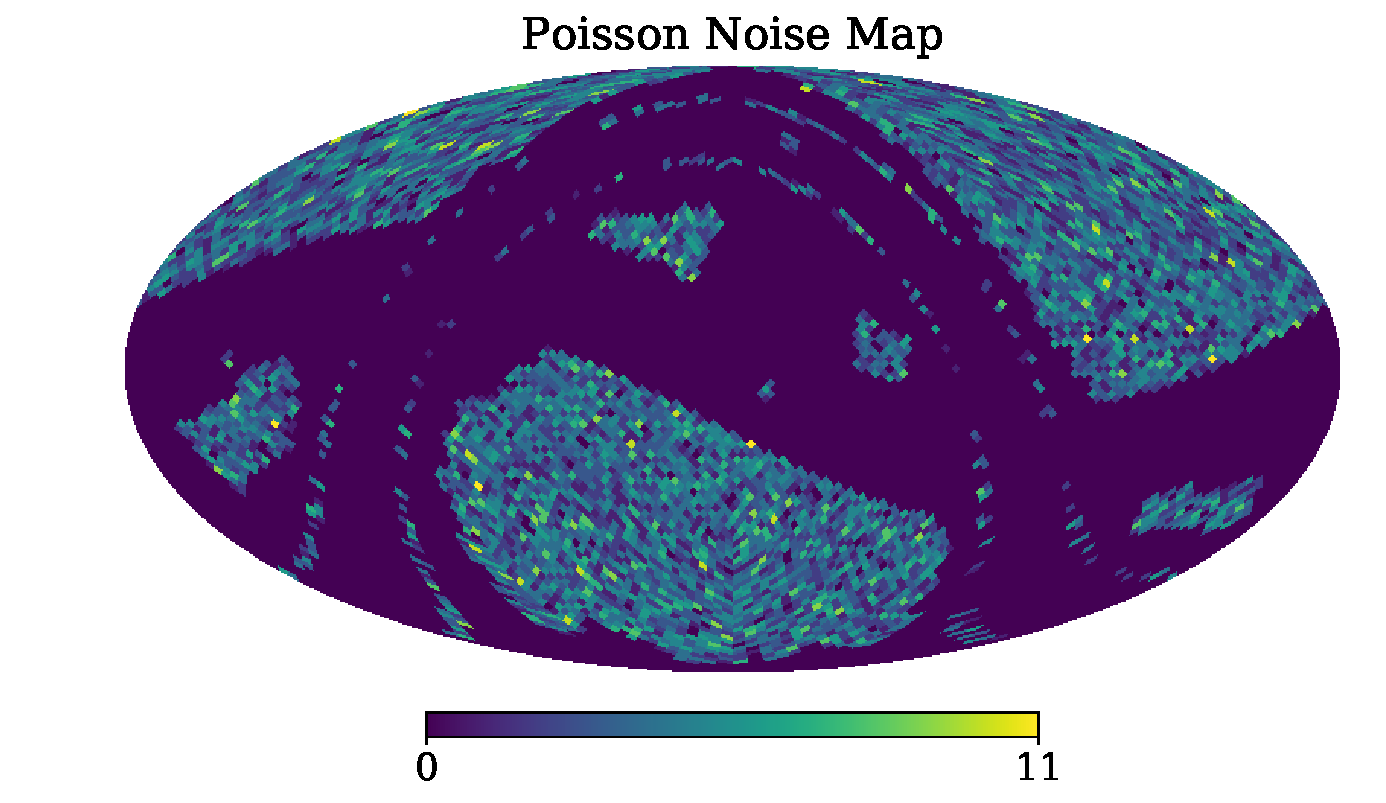
\includegraphics[scale=0.35]{BPL-FIGS/Euclid-NoiseMap-N32.pdf}
  \caption{}
  \label{fig:BPL:LN-LowSN-noise}
\end{subfigure}\\
\begin{subfigure}{.5\textwidth}
  \centering
  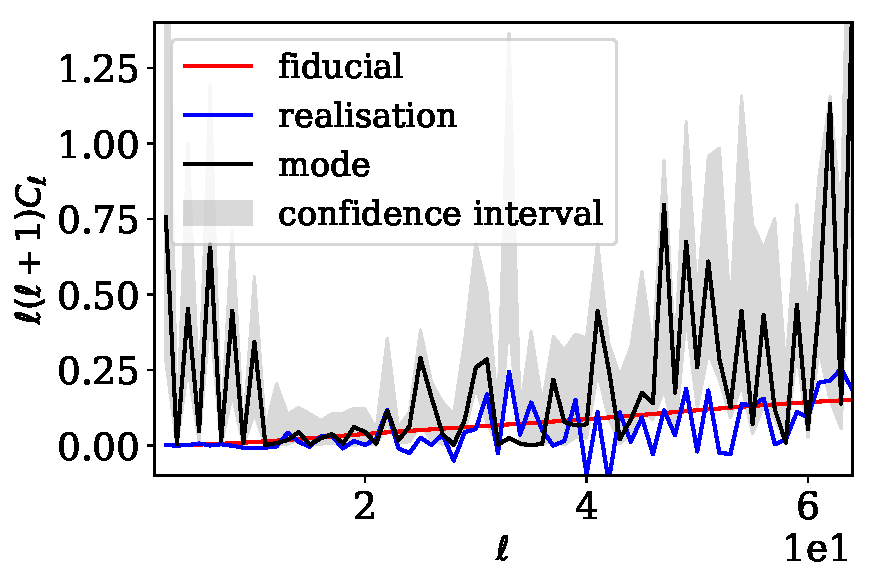
\includegraphics[scale=0.50]{BPL-FIGS/Euclid-Foot-LN-PoiNoi-N32_HPDCls.pdf}
  \caption{}
  \label{fig:BPL:LN-LowSN-Cls}
\end{subfigure}
\begin{subfigure}{.5\textwidth}
  \centering
  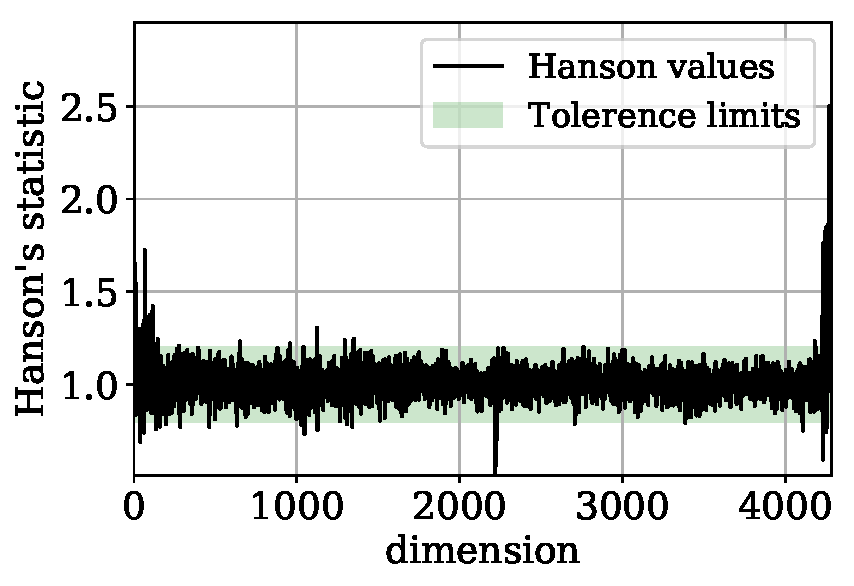
\includegraphics[scale=0.50]{BPL-FIGS/Euclid-Foot-LN-PoiNoi-N32_Hanson.pdf}
    \caption{}
    \label{fig:BPL:LN-LowSN-Hanson}
\end{subfigure}
\caption[Bayesian-$C_{\ell}$ estimator tested on a Euclid-like \flask log-normal simulation with low signal-to-noise.]{\textit{(a)} Log-normal simulation with a Poissonian noise realisation generated with \flask for galaxy clustering using an Euclid-like mask (see Figure \ref{fig:BPL:EuclidMask}). \textit{(b)} Inverse-noise map used in the Bayesian estimator for the analysis. Here, $\bar{n}^{-1}\approx 2.85\times 10^{-4}$ steradians/galaxies. \textit{(c)} Results from the Bayesian-$C_{\ell}$ estimator tests. The red line shows the fiducial angular power spectrum used to generate the simulation, blue line shows the results obtained with the Pseudo-$C_{\ell}$ estimator. Finally, the black line is the mode of the Bayesian estimator samples and the shaded region shows the 68\% confidence regions from the sampled posterior. \textit{(d)} Hanson test demonstrating an acceptable convergence is able to recover the fiducial power spectrum with satisfactory accuracy. Results here were obtained with $N_{samples} = 335,000$.}
\label{fig:BPL:LogNormalFSAnalysis}
\end{figure}

\begin{figure}
\begin{subfigure}{.5\textwidth}
  \centering
  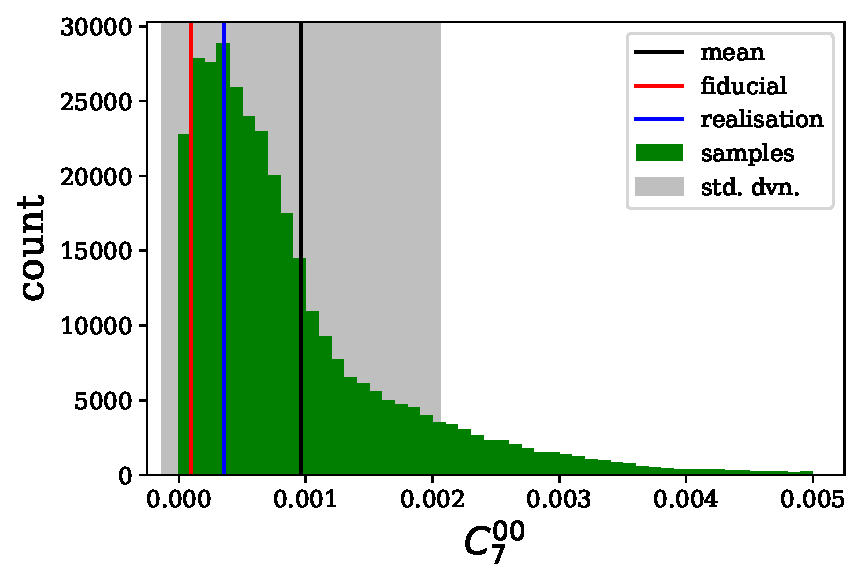
\includegraphics[scale=0.50]{BPL-FIGS/Euclid-foot-LN-PoiNoi-N32-HISTOGRAM-ell-07.pdf}
  \caption{$\ell = 7$}
\end{subfigure}
\begin{subfigure}{.5\textwidth}
  \centering
  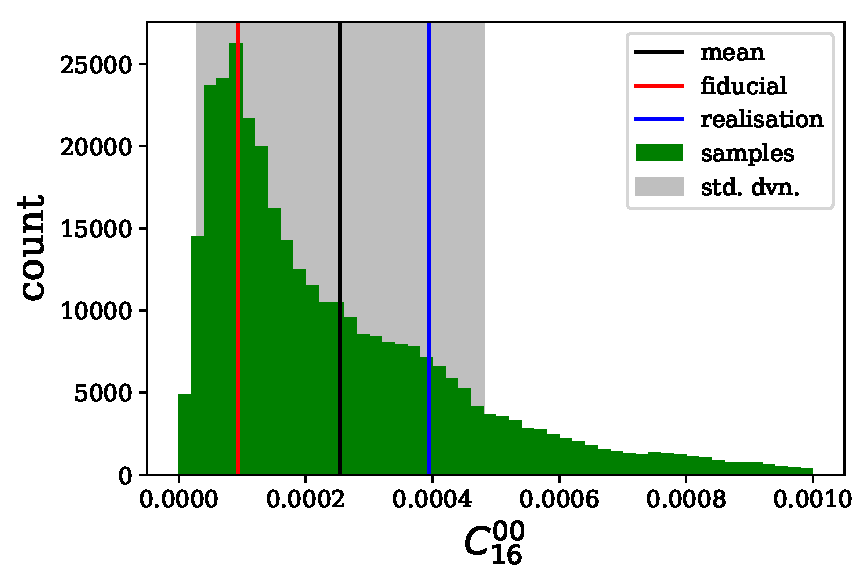
\includegraphics[scale=0.50]{BPL-FIGS/Euclid-foot-LN-PoiNoi-N32-HISTOGRAM-ell-16.pdf}
  \caption{$\ell = 16$}
\end{subfigure}
\begin{subfigure}{.5\textwidth}
  \centering
  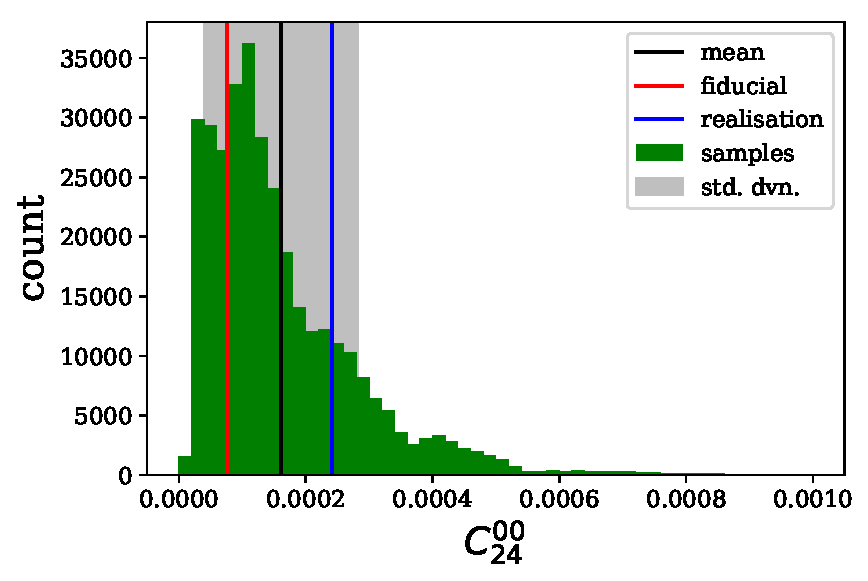
\includegraphics[scale=0.50]{BPL-FIGS/Euclid-foot-LN-PoiNoi-N32-HISTOGRAM-ell-24.pdf}
  \caption{$\ell = 24$}
\end{subfigure}
\begin{subfigure}{.5\textwidth}
  \centering
  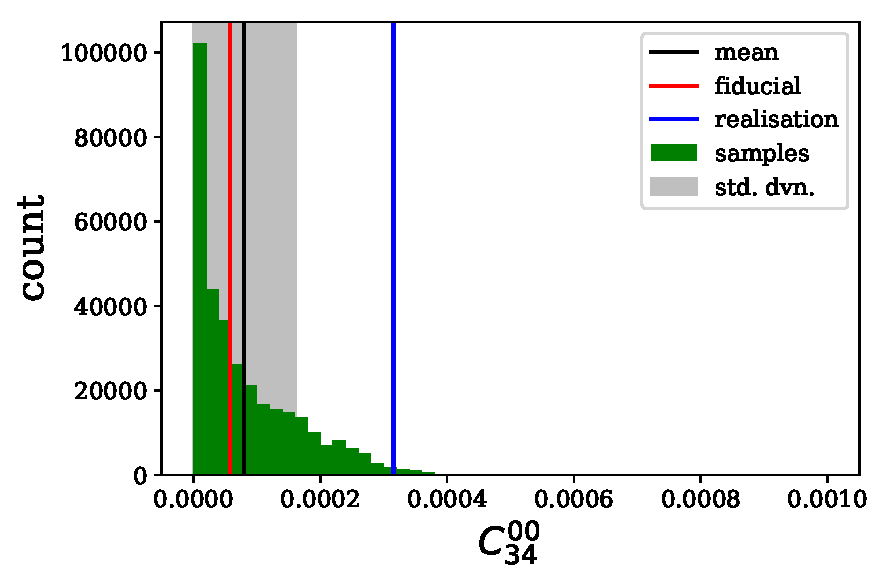
\includegraphics[scale=0.50]{BPL-FIGS/Euclid-foot-LN-PoiNoi-N32-HISTOGRAM-ell-34.pdf}
  \caption{$\ell = 34$}
\end{subfigure}
\begin{subfigure}{.5\textwidth}
  \centering
  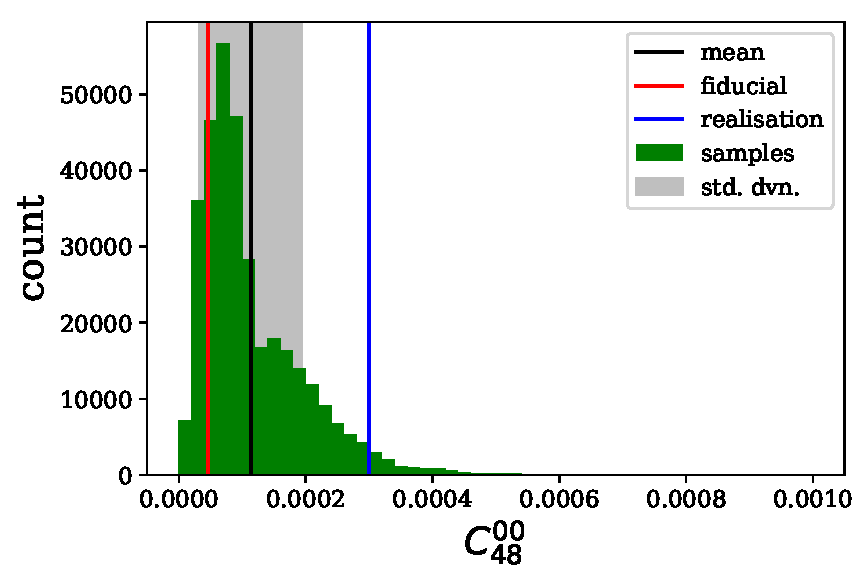
\includegraphics[scale=0.50]{BPL-FIGS/Euclid-foot-LN-PoiNoi-N32-HISTOGRAM-ell-48.pdf}
  \caption{$\ell = 48$}
\end{subfigure}
\begin{subfigure}{.5\textwidth}
  \centering
  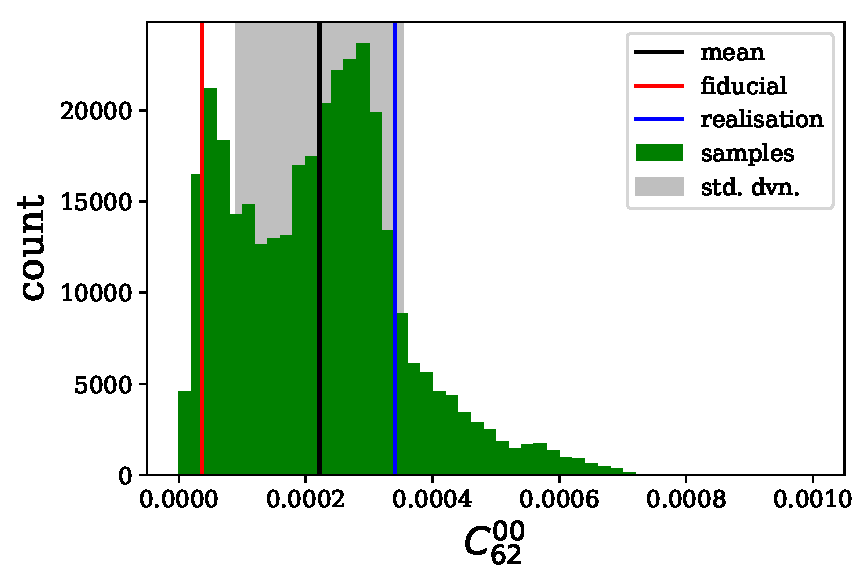
\includegraphics[scale=0.50]{BPL-FIGS/Euclid-foot-LN-PoiNoi-N32-HISTOGRAM-ell-62.pdf}
  \caption{$\ell = 62$}
\end{subfigure}
\caption[Examples of marginalised 1D posteriors for individual $\ell$-modes for the case of a Euclid-like mask and a very low signal-to-noise.]{Examples of the marginalised 1D posteriors for individual $\ell$-modes for the case of a Euclid-like mask and a very low signal-to-noise, $\bar{n}^{-1}\approx 2.85\times 10^{-4}$ steradians/galaxies. Note that some cases exhibit a secondary peak, like in the \textit{(f)} panel, which coincides with the value estimated by the Pseudo-$C_{\ell}$ estimator. Even though in some cases the mean and standard deviation of the samples are far away from the fiducial value, the peak is at the correct value in most cases.}
\label{fig:BPL:Euclid-Ells}
\end{figure}

\qquad Next, the final log-normal simulation to be studied in this section has a signal-to-noise similar to the expected from Euclid's galaxy clustering measurements at the given redshift range, e. g. $\bar{n}^{-1}\approx 2.86\times 10^{-8}$ steradians/galaxies \citep{2011EuclidRedPaper}. The simulated overdensity map and the galaxy number counts map used as a proxy for inverse noise are shown in Figures \ref{fig:BPL:LN-HighSN-dens} and \ref{fig:BPL:LN-HighSN-noise}, respectively. Note that the values in the inverse-noise map contains many more galaxies than the previous case. For this case, shown in Figure \ref{fig:BPL:LN-HighSN-Cls}, one can see that the recovered angular power spectrum using the Bayesian estimator looks closer to the fiducial $C_{\ell}$s. 

\qquad Note how, given the higher signal-to-noise in this simulation, even with values for the Hanson test above the tolerance levels (see Figure \ref{fig:BPL:LN-HighSN-Hanson} and Section \ref{Sec:BPL:Convergence}), satisfactory convergence in the chains was achieved with impressive accuracy and precision using 435,000 samples. The marginalised $C_{\ell}$ for each individual $\ell$-mode, presented in Figure \ref{fig:BPL:Euclid-Ells-HighSN} for this case, demonstrate how the posterior distribution was properly sampled in this case. For the larger scales, the distribution of sampled $C_{\ell}$s is very skewed and, as expected, as one looks at smaller scales, the $\chi$-squared distributed $C_{\ell}$s tend to a Gaussian distribution. This has great implications as it demonstrates that the method recovers non-Gaussian error-bars for the low-$\ell$ modes, being a great advantage over method such as Pseudo-$C_{\ell}$ or other quadratic estimators \citep{Boris2013}.

\begin{figure}
\begin{subfigure}[b]{.5\textwidth}
 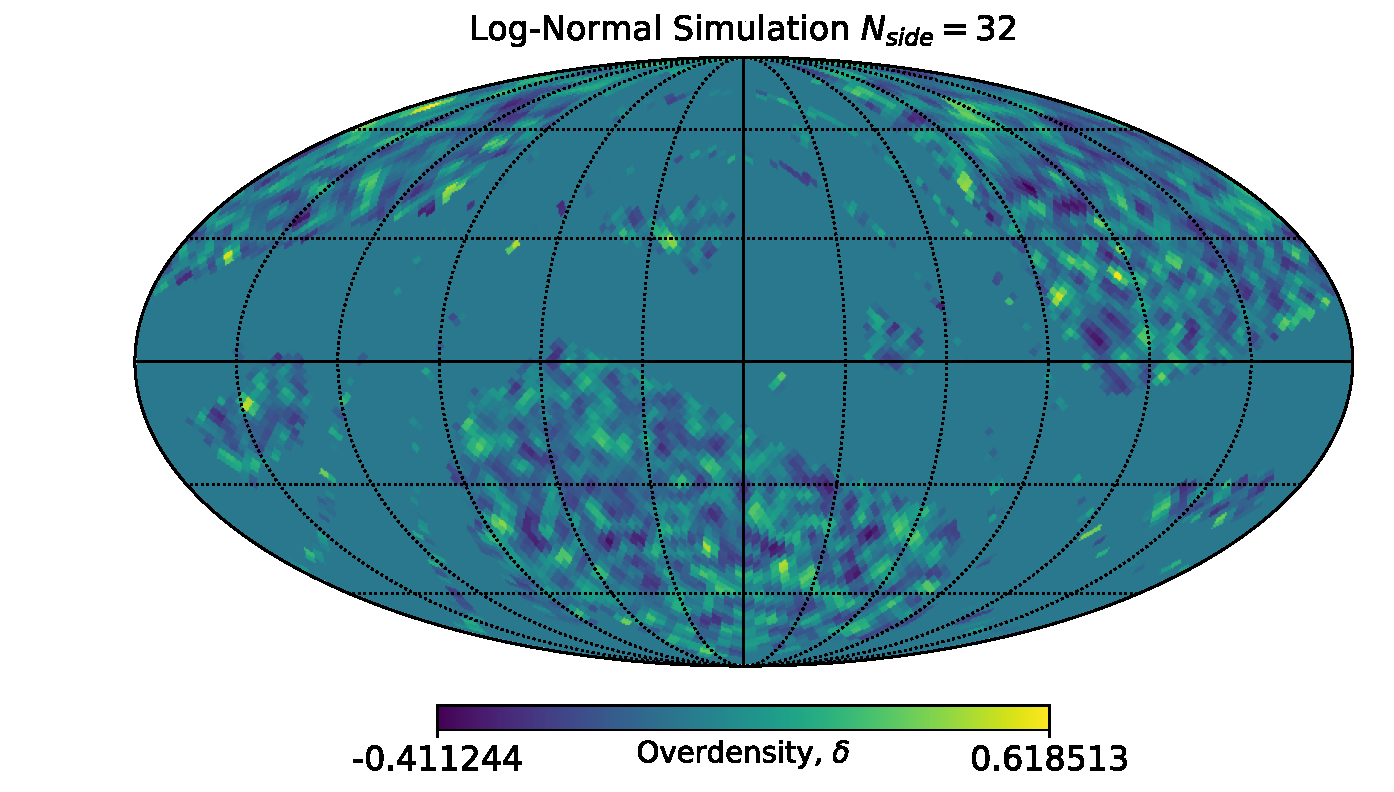
\includegraphics[scale=0.34]{BPL-FIGS/Euclid-LN-PNoi-N32-HDens_map.pdf}
  \caption{}
  \label{fig:BPL:LN-HighSN-dens}
\end{subfigure}
\begin{subfigure}[b]{.5\textwidth}
 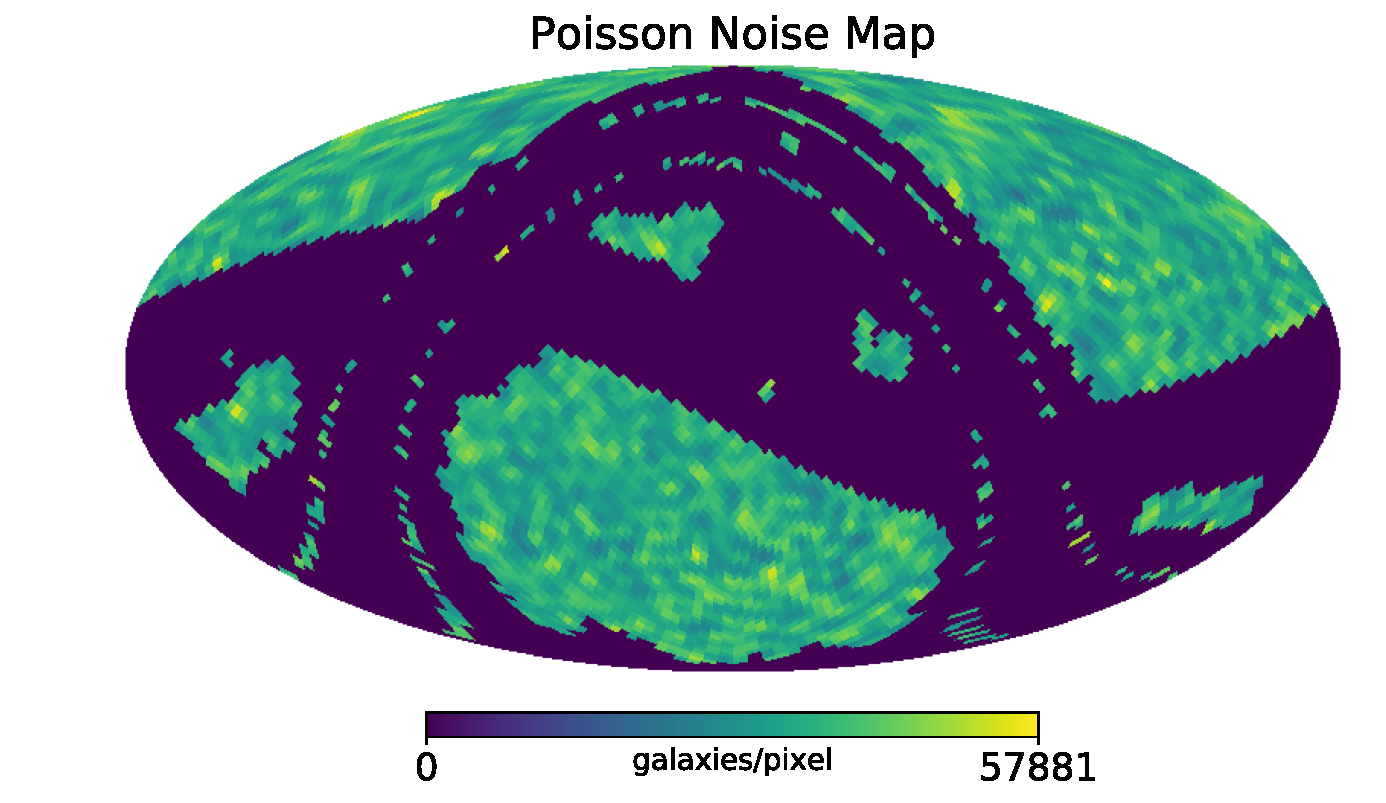
\includegraphics[scale=0.34]{BPL-FIGS/Euclid-LN-PNoi-N32-NoiseMap.pdf}
  \caption{}
  \label{fig:BPL:LN-HighSN-noise}
\end{subfigure}\\
\begin{subfigure}{.5\textwidth}
  \centering
  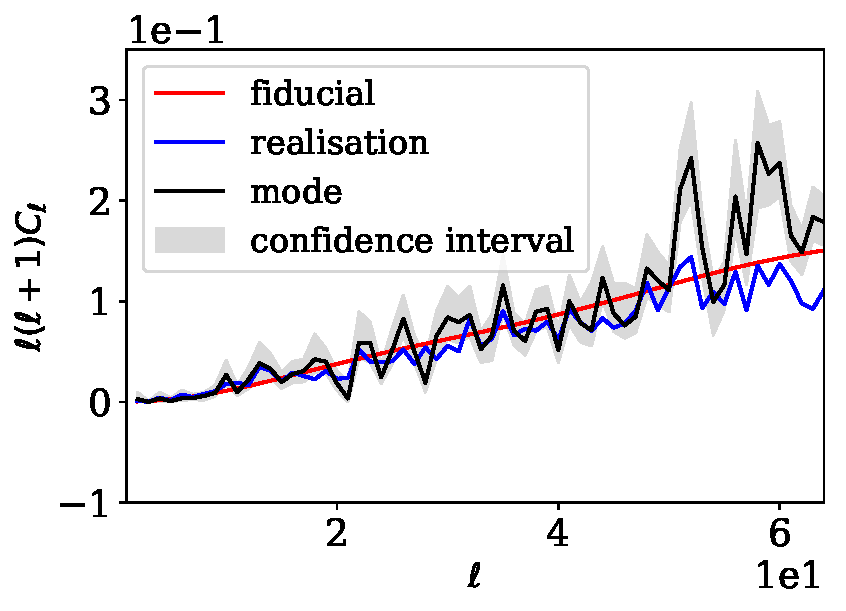
\includegraphics[scale=0.50]{BPL-FIGS/Euclid-LN-PNoi-N32-HDens_HPDCls.pdf}
  \caption{}
  \label{fig:BPL:LN-HighSN-Cls}
\end{subfigure}
\begin{subfigure}{.5\textwidth}
  \centering
  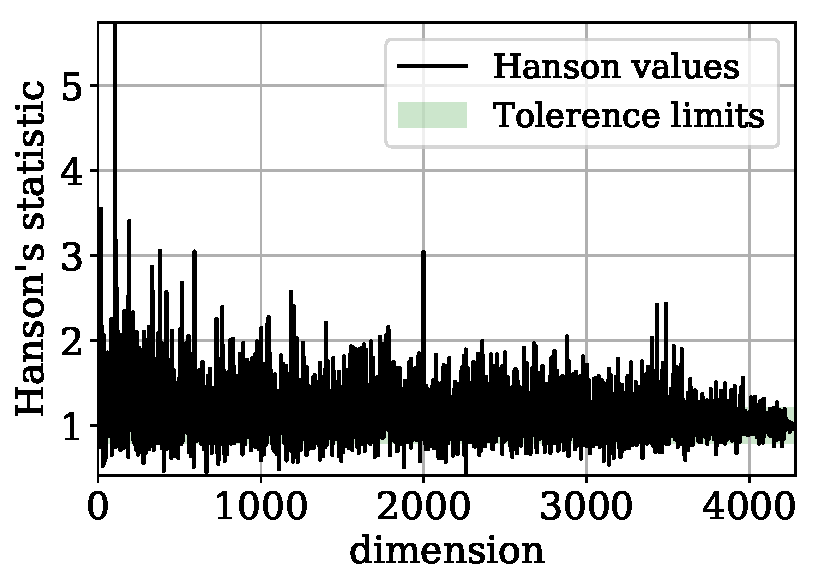
\includegraphics[scale=0.50]{BPL-FIGS/Euclid-LN-PNoi-N32-HDens_Hanson.pdf}
  \caption{}
  \label{fig:BPL:LN-HighSN-Hanson}
\end{subfigure}
\caption[Bayesian-$C_{\ell}$ estimator tested on a Euclid-like \flask log-normal simulation with signal-to-noise similar to Euclid's.]{\textit{(a)} Log-normal simulation with a Poissonian noise realisation generated with \flask for galaxy clustering using an Euclid-like mask (see Figure \ref{fig:BPL:EuclidMask}) and redshift distribution. \textit{(b)} Inverse-noise map used in the Bayesian estimator for the analysis with $\bar{n}^{-1}\approx 2.86\times 10^{-8}$ steradians/galaxies -- which is close to forecasts for Euclid \citep{2011EuclidRedPaper,2017EuclidLSST}. \textit{(c)} Results from the Bayesian-$C_{\ell}$ estimator tests. The red line shows the fiducial angular power spectrum used to generate the simulation, blue line shows the results obtained with the Pseudo-$C_{\ell}$ estimator. Black line is the mode of the Bayesian estimator samples and the shaded region shows the 68\% confidence regions from the sampled posterior, after marginalising over the $a_{\ell m}$ coefficients. \textit{(d)} Hanson test: here, it looks at first instance that the chain is still not converged. However, as this case contains a higher signal-to-noise ratio, the marginalised posteriors are converged as it can be seen in Figure \ref{fig:BPL:Euclid-Ells-HighSN}. Results were obtained with $N_{samples} = 435,000$.}
\label{fig:BPL:LogNormalFSAnalysisHighSN}
\end{figure}


\qquad Results from Figures \ref{fig:BPL:LogNormalFSAnalysisHighSN} and \ref{fig:BPL:Euclid-Ells-HighSN} demonstrate that, for an Euclid-like survey, in a single shell case, the Bayesian estimator presented in this chapter can properly recover the underlying angular power spectrum of galaxies. The performance of the method was enhanced by using the galaxy number counts map as a proxy for the inverse-noise map; without it, the algorithm can get lost in local maxima inside the prior. Tests will be perform in the future for cases with more than one shell and cross-correlations between shells.


\begin{figure}
\begin{subfigure}{.5\textwidth}
  \centering
  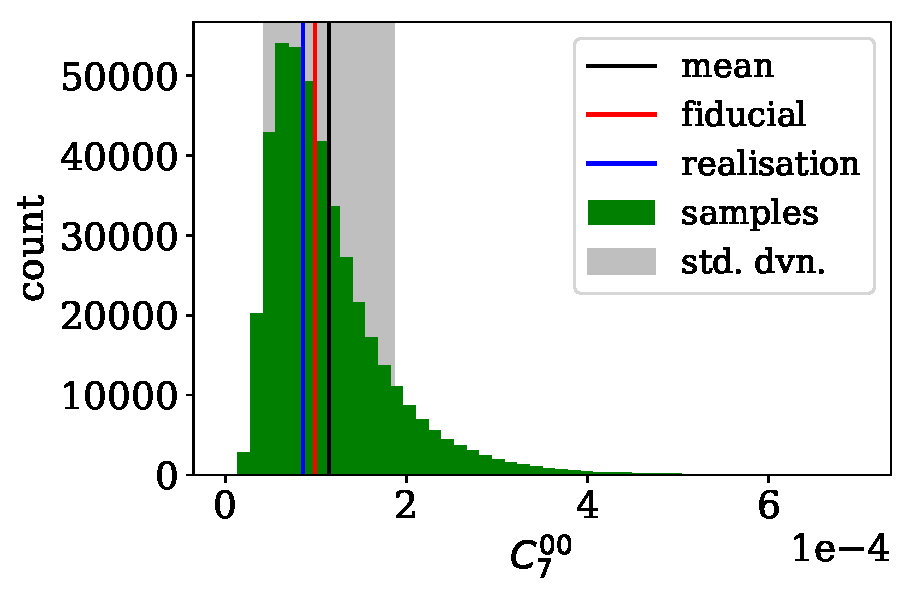
\includegraphics[width=\textwidth]{BPL-FIGS/Euclid-LN-PNoi-N32-HDens_HISTOGRAM-ell-07.pdf}
  \caption{$\ell = 7$}
\end{subfigure}
\begin{subfigure}{.5\textwidth}
  \centering
  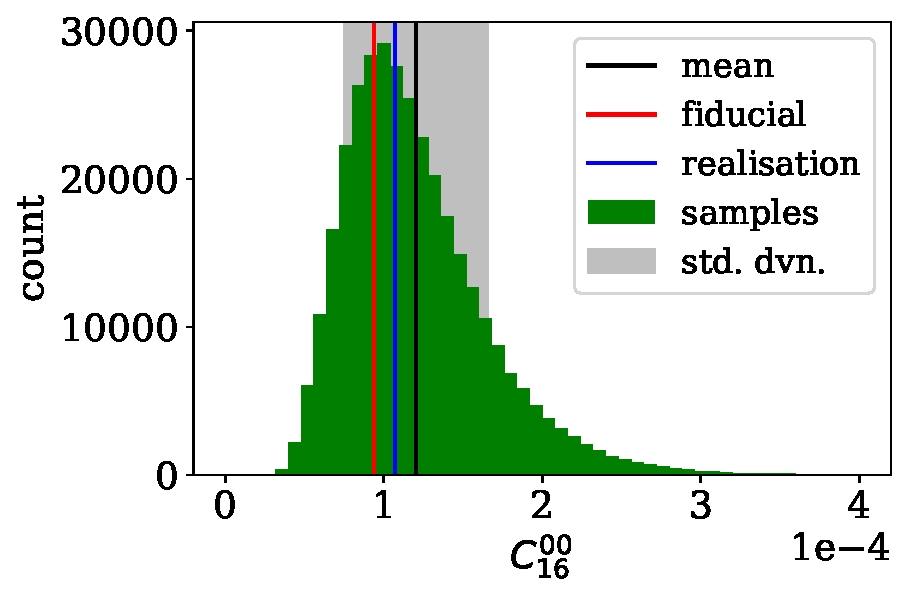
\includegraphics[width=\textwidth]{BPL-FIGS/Euclid-LN-PNoi-N32-HDens_HISTOGRAM-ell-16.pdf}
  \caption{$\ell = 16$}
\end{subfigure}
\begin{subfigure}{.5\textwidth}
  \centering
  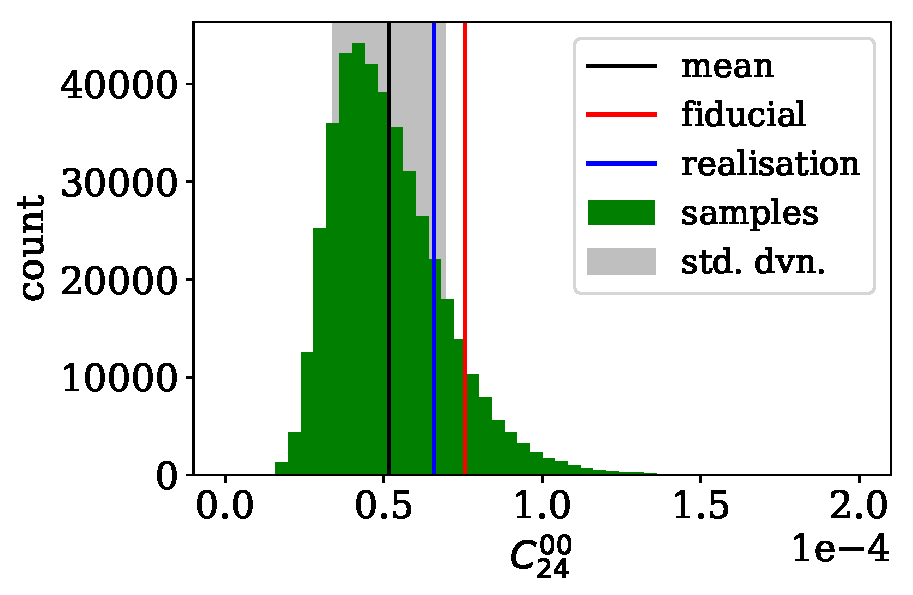
\includegraphics[width=\textwidth]{BPL-FIGS/Euclid-LN-PNoi-N32-HDens_HISTOGRAM-ell-24.pdf}
  \caption{$\ell = 24$}
\end{subfigure}
\begin{subfigure}{.5\textwidth}
  \centering
  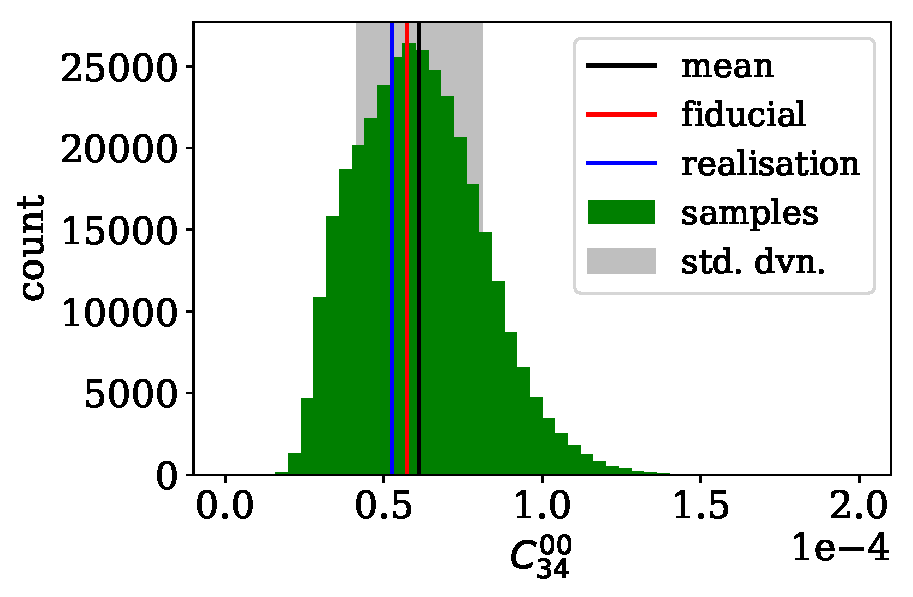
\includegraphics[width=\textwidth]{BPL-FIGS/Euclid-LN-PNoi-N32-HDens_HISTOGRAM-ell-34.pdf}
  \caption{$\ell = 34$}
\end{subfigure}
\begin{subfigure}{.5\textwidth}
  \centering
  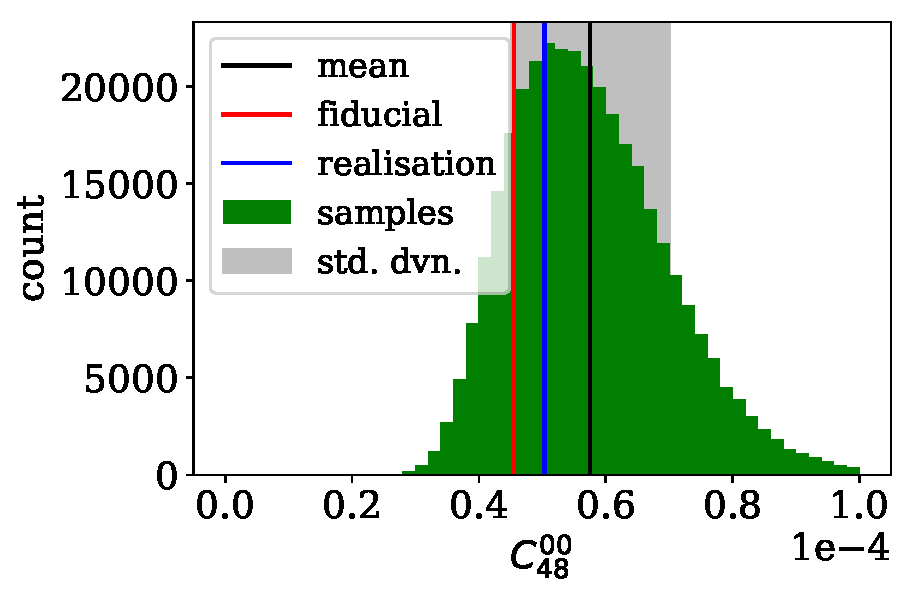
\includegraphics[width=\textwidth]{BPL-FIGS/Euclid-LN-PNoi-N32-HDens_HISTOGRAM-ell-48.pdf}
  \caption{$\ell = 48$}
\end{subfigure}
\begin{subfigure}{.5\textwidth}
  \centering
  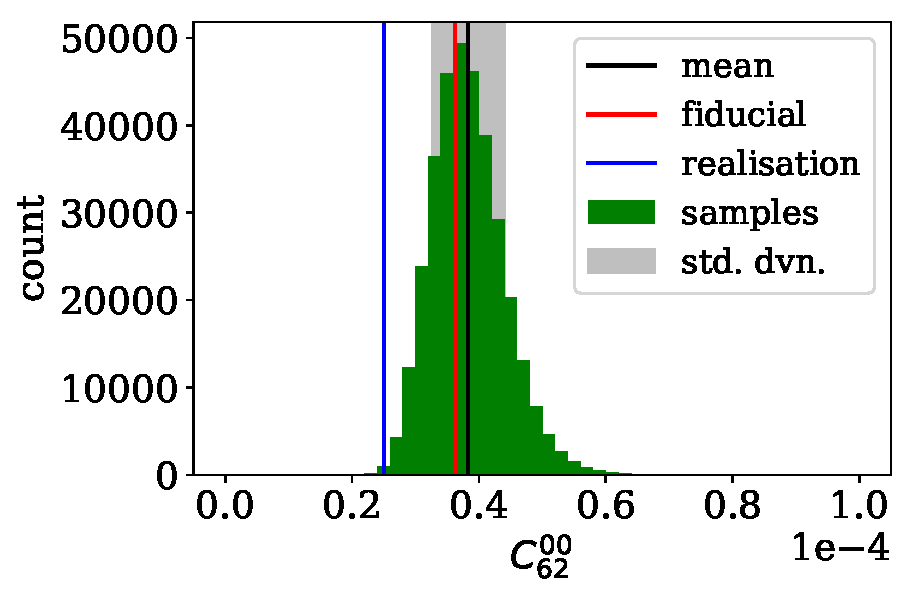
\includegraphics[width=\textwidth]{BPL-FIGS/Euclid-LN-PNoi-N32-HDens_HISTOGRAM-ell-62.pdf}
  \caption{$\ell = 62$}
\end{subfigure}
\caption[Examples of marginalised 1D posteriors for individual $\ell$-modes for the case of a Euclid-like mask and signal-to-noise.]{Examples of the marginalised 1D posteriors for individual $\ell$-modes for the case of a Euclid-like mask and signal-to-noise, $\bar{n}^{-1}\approx 2.86\times 10^{-8}$ steradians/galaxies. For this situation, one can observe how the high-$\ell$ mode present a more Gaussian-like distribution as the low-$\ell$ modes are much more skewed. In most cases, the marginalised posterior's peak is matching the input fiducial $C_{\ell}$.}
\label{fig:BPL:Euclid-Ells-HighSN}
\end{figure}




%\subsection{Investigation of the Hessian's impact}
% \textcolor{red}{Nside = 1024 Number of Shells = 2}

% Brief explanation of how Flask works.
% \subsection{Full-Sky}
% \begin{itemize}
% \item  Spin 0
% \item  Spin 2
% \item  Low and High S/N Regimes
% \item  \textcolor{blue}{Figure of the maps}
% \end{itemize}

% \subsection{Euclid-Like case:}
% \begin{itemize}
% \item  Nside and Nshells
% \item Explain the Mask used
% \item  Spin 0 (LSS)  + Spin 2 (Shear)
% \item  \textcolor{blue}{Figure of the maps}
% \end{itemize}

% %----------------------------------------------------------------%
% %                        MEASUREMENTS FROM SIMULATIONS
% %---------------------------------------------------------------%
% \section{Measurements from the Simulations}
% \begin{itemize}
% \item (Spin 0, 2, 0x2);
% \item  Euclid-Like (Spin 0, 2, 0x2)
% \item  Show  marginalised  1D  $\ell$'s
% \item  \textcolor{red}{Comparison w/ PCL? YES! ---> WE HAVE NO PCL FOR WEAK-LENSING!}
% \item \textcolor{blue}{Figures}
% \end{itemize}

%----------------------------------------------------------------%
%                        	CONCLUSIONS 
%----------------------------------------------------------------%
\section{Conclusions and Future Applications}
In this investigative Chapter, I have presented the formalism to generically estimate angular power spectra for both spin-0 and spin-2 fields as outlined in the literature \citep{Borrill1999, Hobson2002, Taylor2008,SreeThesis}. I have then presented how to use a Guided Hamiltonian Monte-Carlo for sampling such high dimensional posterior distributions, $\mathcal{O}(10^{4}-10^{7})$ dimensions, and the approximations taken when obtaining the Hessian of the posterior, as a part of the GHS. Even though it seemed simple at first, applying the methodology outlined in Section \ref{Sec:BPL:Modeling} to galaxy clustering proved to be more complex than expected. This was a very time consuming and complicated project, leading to a chapter with partial results but with extreme potential for extensions in the near future. Due to time constraints, I could not extend the work perform here for weak lensing shear measurements -- this is now a part of the scope of my work as an Euclid Research Assistant. 

\qquad I have presented here the nuisances and important details to apply this Bayesian-$C_{\ell}$ estimator to galaxy clustering samples. I demonstrated that the method works for both Gaussian and log-normal full sky simulations with little to no difference.\footnote{This was already demonstrated for Gaussian simulations in \cite{SreeThesis}, but never in log-normal simulations with Poissonian noise -- as in galaxy clustering.} I have then pursued to investigate the impact of survey's geometries in introducing correlations between the spherical harmonic coefficients and the impact such correlations have in estimating the angular power spectra of galaxies. Finally, I apply the method for Euclid-like log-normal simulations, for an intermediate redshift range, probing large scales $l_{max} \leq 64$. Two different signal-to-noise scenarios were investigated with the best results coming from the case that is closer to Euclid's future galaxy cluster sample: one with a similar galaxy density as expected for Euclid and a case with $10^{4}$ less galaxies. The estimator performed well in both cases, with an increase of accuracy in the first case. However, it is important to note that, for the GHS Bayesian estimator to work properly in the case of galaxy clustering in a cut-sky scenario, one has to consider noise to anisotropic, i. e. one has to use the galaxy number count map as a proxy for the inverse-noise map in the method.

\qquad Following, when observing the marginalised posteriors for each mode (Figure \ref{fig:BPL:Euclid-Ells-HighSN}), it is possible to see that the samples recover the correct posterior distribution, allowing to probe the $\chi$-square nature of low-$\ell$ mode's distributions. This improves not only accuracy but also precision on $C_{\ell}$ estimates. Usual approaches taken by the community -- Pseudo-$C_{\ell}$ or Quadratic Maximum Likelihood estimators -- assume symmetrical uncertainties even for the large scale modes, even though we know that statistically that is not the case. This makes the Bayesian-$C_{\ell}$ estimator an important tool when probing large scales, which are fundamental for probing primordial non-Gaussianities, through $f_{nl}$ measurements, with future galaxy surveys. Probing these large scales with a Pseudo-$C_{\ell}$ estimator can be very tricky -- as shown in Chapter \ref{Chap:BOSS}. 

\qquad Another important remark related to this methodology, note that since one is obtaining samples for the power spectrum, it is possible to estimate uncertainties with no need for mocks or N-body simulations. These remarks lead to an interesting debate related to measuring cosmological parameters from Bayesian-$C_{\ell}$ estimates. Here, I propose that two approaches can be taken -- and both need further investigation. The simplest one would be to obtain a covariance matrix from the samples itself and perform an analysis similar to the one presented in Section \ref{Sec:CosmoAnal}, i. e. ignoring the information related to the posterior value for each of the sampled points. A second and more powerful approach would be to perform a N-dimensional interpolation in the sampled posterior values -- possibly with the use of kernel density estimation or machine learning methods. Using this high dimensional posterior, one can use theoretical prediction for $C_{\ell}$ given sampled cosmological parameters. These can then be compare to the posterior value from the estimated angular power spectra using this advanced interpolation technique. This would result in a fully hierarchical Bayesian method to obtain cosmological parameters from measurements of the angular power spectra of galaxies. 

\qquad Finally, when extending this approach to weak lensing shear measurements, this method has the potential to simultaneously probe the angular power spectra of cosmic shear while also providing the tools to estimate cosmic mass maps. Since the method probes both $C_{\ell}$s and $a_{\ell m}$ coefficients, the latter can be use to estimate the dark matter mass distribution via mass map reconstructions \citep{2018Niall}. The formalism here is not very different from the one developed in \cite{AlmostBlackPearl2016}, which a difference that the method would then work in a curved sky situation. Parallel effort is being made in this project in order to modify the method to obtain mass maps.